\documentclass[12pt,twoside]{report}
%\documentclass[conference]{IEEEtran}
%%%%%%%%%%%%%%%%%%%%%%%%%%%%%%%%%%%%%%%%%%%%%%%%%%%%%%%%%%%%%%%%%%%%%%%%%%%%%

% Definitions for the title page
% Edit these to provide the correct information
% e.g. \newcommand{\reportauthor}{Timothy Kimber}

\newcommand{\reporttitle}{I need a title}
\newcommand{\reportauthor}{Tianyang Sun}
\newcommand{\supervisor}{Dr Benny Lo}
\newcommand{\degreetype}{MSc Computing}

%%%%%%%%%%%%%%%%%%%%%%%%%%%%%%%%%%%%%%%%%%%%%%%%%%%%%%%%%%%%%%%%%%%%%%%%%%%%%

% load some definitions and default packages
%%%%%%%%%%%%%%%%%%%%%%%%%%%%%%%%%%%%%%%%%
% University Assignment Title Page 
% LaTeX Template
% Version 1.0 (27/12/12)
%
% This template has been downloaded from:
% http://www.LaTeXTemplates.com
%
% Original author:
% WikiBooks (http://en.wikibooks.org/wiki/LaTeX/Title_Creation)
%
% License:
% CC BY-NC-SA 3.0 (http://creativecommons.org/licenses/by-nc-sa/3.0/)
% 
%
%%%%%%%%%%%%%%%%%%%%%%%%%%%%%%%%%%%%%%%%%
%----------------------------------------------------------------------------------------
%	PACKAGES AND OTHER DOCUMENT CONFIGURATIONS
%----------------------------------------------------------------------------------------
\usepackage[a4paper,hmargin=2.8cm,vmargin=2.0cm,includeheadfoot]{geometry}
\usepackage{textpos}
\usepackage[numbers]{natbib} % for bibliography
\usepackage{tabularx,longtable,multirow,subfigure,caption}%hangcaption
\usepackage{fncylab} %formatting of labels
\usepackage{fancyhdr} % page layout
\usepackage{url} % URLs
\usepackage[english]{babel}
\usepackage{amsmath}
\usepackage{graphicx}
\usepackage{dsfont}
\usepackage{epstopdf} % automatically replace .eps with .pdf in graphics
\usepackage{backref} % needed for citations
\usepackage{array}
\usepackage{latexsym}
\usepackage[pdftex,pagebackref,hypertexnames=false,colorlinks]{hyperref} % provide links in pdf
%\usepackage{biblatex}
\usepackage{multirow}

\hypersetup{pdftitle={},
  pdfsubject={}, 
  pdfauthor={},
  pdfkeywords={}, 
  pdfstartview=FitH,
  pdfpagemode={UseOutlines},% None, FullScreen, UseOutlines
  bookmarksnumbered=true, bookmarksopen=true, colorlinks,
    citecolor=black,%
    filecolor=black,%
    linkcolor=black,%
    urlcolor=black}

\usepackage[all]{hypcap}
\usepackage{amssymb}
%\usepackage{color}
%\usepackage[tight,ugly]{units}
%\usepackage{float}
%\usepackage{tcolorbox}
%\usepackage[colorinlistoftodos]{todonotes}
% \usepackage{ntheorem}
% \theoremstyle{break}
% \newtheorem{lemma}{Lemma}
% \newtheorem{theorem}{Theorem}
% \newtheorem{remark}{Remark}
% \newtheorem{definition}{Definition}
% \newtheorem{proof}{Proof}


%%% Default fonts
\renewcommand*{\rmdefault}{bch}
\renewcommand*{\ttdefault}{cmtt}



%%% Default settings (page layout)
\setlength{\parindent}{0em}  % indentation of paragraph

\setlength{\headheight}{14.5pt}
\pagestyle{fancy}
\renewcommand{\chaptermark}[1]{\markboth{\chaptername\ \thechapter.\ #1}{}} 

\fancyfoot[ER,OL]{\sffamily\textbf{\thepage}}%Page no. in the left on odd pages and on right on even pages
\fancyfoot[OC,EC]{\sffamily }
\renewcommand{\headrulewidth}{0.1pt}
\renewcommand{\footrulewidth}{0.1pt}
\captionsetup{margin=10pt,font=small,labelfont=bf}


%--- chapter heading

\def\@makechapterhead#1{%
  \vspace*{10\p@}%
  {\parindent \z@ \raggedright \sffamily
    \interlinepenalty\@M
    \Huge\bfseries \thechapter \space\space #1\par\nobreak
    \vskip 30\p@
  }}

%---chapter heading for \chapter*  
\def\@makeschapterhead#1{%
  \vspace*{10\p@}%
  {\parindent \z@ \raggedright
    \sffamily
    \interlinepenalty\@M
    \Huge \bfseries  #1\par\nobreak
    \vskip 30\p@
  }}

\allowdisplaybreaks

% load some macros
% Here, you can define your own macros. Some examples are given below.

\newcommand{\R}[0]{\mathds{R}} % real numbers
\newcommand{\Z}[0]{\mathds{Z}} % integers
\newcommand{\N}[0]{\mathds{N}} % natural numbers
\newcommand{\C}[0]{\mathds{C}} % complex numbers
\renewcommand{\vec}[1]{{\boldsymbol{{#1}}}} % vector
\newcommand{\mat}[1]{{\boldsymbol{{#1}}}} % matrix


\date{June 2020}

\begin{document}

% load title page
% Last modification: 2015-08-17 (Marc Deisenroth)
\begin{titlepage}

\newcommand{\HRule}{\rule{\linewidth}{0.5mm}} % Defines a new command for the horizontal lines, change thickness here


%----------------------------------------------------------------------------------------
%	LOGO SECTION
%----------------------------------------------------------------------------------------


\includegraphics[width = 4cm]{./figures/imperial}\\[0.5cm] 

\center % Center remainder of the page

%----------------------------------------------------------------------------------------
%	HEADING SECTIONS
%----------------------------------------------------------------------------------------

\textsc{\Large Imperial College London}\\[0.5cm] 
\textsc{\large Department of Computing}\\[0.5cm] 

%----------------------------------------------------------------------------------------
%	TITLE SECTION
%----------------------------------------------------------------------------------------

\HRule \\[0.4cm]
{ \huge \bfseries \reporttitle}\\ % Title of your document
\HRule \\[1.5cm]
 
%----------------------------------------------------------------------------------------
%	AUTHOR SECTION
%----------------------------------------------------------------------------------------

\begin{minipage}{0.4\textwidth}
\begin{flushleft} \large
\emph{Author:}\\
\reportauthor % Your name
\end{flushleft}
\end{minipage}
~
\begin{minipage}{0.4\textwidth}
\begin{flushright} \large
\emph{Supervisor:} \\
\supervisor % Supervisor's Name
\end{flushright}
\end{minipage}\\[4cm]


%----------------------------------------------------------------------------------------
%	FOOTER & DATE SECTION
%----------------------------------------------------------------------------------------
%\vfill % Fill the rest of the page with whitespace
%Submitted in partial fulfillment of the requirements for the MSc degree in
%\degreetype~of Imperial College London\\[0.5cm]

\makeatletter
\@date 
\makeatother


\end{titlepage}



% page numbering etc.
\pagenumbering{roman}
\clearpage{\pagestyle{empty}\cleardoublepage}
\setcounter{page}{1}
\pagestyle{fancy}

\begin{abstract}
Your abstract.
\end{abstract}

\cleardoublepage
%%%%%%%%%%%%%%%%%%%%%%%%%%%%%%%%%%%%
\section*{Acknowledgments}
Comment this out if not needed.

\clearpage{\pagestyle{empty}\cleardoublepage}


%%%%%%%%%%%%%%%%%%%%%%%%%%%%%%%%%%%%
%--- table of contents
\fancyhead[RE,LO]{\sffamily {Table of Contents}}
\tableofcontents 


\clearpage{\pagestyle{empty}\cleardoublepage}
\pagenumbering{arabic}
\setcounter{page}{1}
\fancyhead[LE,RO]{\slshape \rightmark}
\fancyhead[LO,RE]{\slshape \leftmark}


%%%%%%%%%%%%%%%%%%%%%%%%%%%%%%%%%%%%
\chapter{Introduction}

\section{Small sample segmentation}
Deep learning society has witnessed great progress in various kinds of tasks using deep convolutional models in the past decade. The emergence of large-scale dataset such as ImageNet \footnote{http://www.image-net.org/}, CIFAR \footnote{https://www.cs.toronto.edu/~kriz/cifar.html} and COCO \footnote{https://cocodataset.org/\#home} provide relatively a variety of data as well as useful deep learning benchmarks for training complicated deep learning architectures.\\

However, this is not necessarily the case in the medical domain where carefully collected and labelled data is available or published. One common issue in medical segmentation is that the data and its annotation acquiring is time consuming and also more sensitive to individual difference. A common scenario in medical imaging domain is that only a small number of annotated data is available for training and evaluation. A relaxed case is when a relatively larger amounts of unlabelled data is obtained but without expert labeling. The two scenario brings us to two problem set up: \textbf{Supervised segmentation} and \textbf{Semi-supervise segmentation}.

\section{Motivation of the task}
The on going pandemic of coronavirus from winter 2019 till summer 2020 (Covid-19) attract much attention in the medical artificial intelligence domain. Reverse Transcription-Polymerase Chain Reaction (PT-PCR) test is so far, considered the gold standard to report if the patient is test positive, while facing the shortage of testing ability especially in the early stage of the Covid-19 outbreak as well as insufficient sensitivity (high false negative rate). Radiometry diagnosis such as CT scans are more approachable and provide a direct insight into the situation of lungs that could help the early diagnosis of suspected infection, as well as providing the change of Ground glass opacity or nodules. At the same time, radiometry study on the effect of Covid-19 on lungs using CT scans reports that lower right lungs is usually easier to be infected compared to other areas such as upper right lungs using group study. Other findings using CT imaging analysis  showed that after patients were cured, the white part in lungs such as ground glass opacity will still increased and gradually slowly absorbed in the following months.\\

While reading and diagnosing interesting area of CT slices that usually contains around 100 slices along the Axial axis is a time consuming process. Thus the medical imaging domain designed and experimented a large amounts of deep neural architectures aiming to help the CT reading process of several disease including Covid-19.\\

Many works have beed published in the fast changing pandemic based on various precious private dataset. However, very few of them, by the time this report was written, was publicly available to the research community. So one question came into our mind is that: \textbf{How would we give reasonably good segmentation of infection areas when only a small amount of data is available?}\\

In the early stage of this project (April to Late June, 2020), we only have access to the Cov-19 Segmentation benchmark which contains 20 Volumes from multiple centers, which brings us the small sample segmentation setup. In late June 2020, MosMed published their CT scans for public research with 50 volumes of annotated thick slice CT scans and around 500 unlabelled confirmed-case CT scans. The publish of this dataset brings us the second task of a semi-supervise setup for segmentation.\\

The aim of our work here, is to explore the domain of \textbf{imperfect dataset segmentation task}, with small sample size or combined with some unlabelled training medical images, and further experiment the method on the ongoing pandemic.

\section{Summarization of our work}
In short, we summarize our \textbf{contributions} as below:
\begin{enumerate}
	\item We designed an experiment that leveraged the SVCCA tool for the segmentation model behavior under supervised small sample segmentation setup.
	\item We built a semi-supervise pipeline that improve the generalizability of segmentation model leveraging more unlabelled data samples.
\end{enumerate}

More specifically, in this project, we dealt with two common scenarios in medical imaging on segmentation task: (1)only a small set of labelled samples are collected, and (2) a small set of labelled data is available and in addition, a relatively larger amounts of data is collected but not labelled.\\

 For case 1, we explored transfer learning using different pre-training method or available pre-trained models. We also tried to understand the network behavior during transfer learning. We described our design of SVCCA setup in \textbf{section 3.2} and showed the results in \textbf{section 4.6}. \\
 \begin{enumerate}
 	\item First, we pre-trained the model on non-Covid Lung volumes to get a pretrained model $F_{pretrained}$
 	\item  Then we performed transfer learning using Covid dataset on the pretrained model weights.
 	\item \textbf{We designed the SVCCA experiment} in which We analyzed the layers behavior during transfer learning to get a further understanding of the Fine-tuned model. 
 \end{enumerate}
 
 For case 2, we further explored the semi-supervise learning. Our design  contains three main parts: \textbf{Coarse segmentation for patches sampling, pseudo label assigning, and Meat-Teacher training.} For pseudo labeling, we designed a method that assign the segmentation label using cosine similarity score from the labeled dataset. We give a more detailed description of our design in \textbf{section 3.3} and the result in \textbf{section 4.7}
 \begin{enumerate}
 	\item First, given a pretrained model A, we fine-tune to get A' on the small set of Covid dataset until the model gives relatively good performance (e.g Dice coefficient over 0.75).
 	\item Next, we randomly crop 120 68 * 68 patches $P_{img}$ from the labelled datset and store the labels $P_{label}$. We randomly crop 32 68 * 68 slices from each volume of the unlabelled dataset.
 	\item Then, we take the encoder part of A'. Given an unlabelled patch $p_{unlabelled}$, we calculate its cosine similarity with each data in $P_{img}$ in the encoded latent space and get the most similar labels $P_{label_{i}}$ with similarity score $S_{i}$. We assign the mask of the labels to the unlabeled images with a similarity score $S_{i}$ for the labels with \textbf{$S_{i} \in [0.87, 0.96]$ }.
 	\item The expert labeled images go through the student network and calculate the segmentation loss $L_{seg}$; The pseudo labeled samples go through the student network for weighted segmentation loss $w \times 0.5 L_{seg}$ of which $w$ is the cosine similarity score, and the teacher network for $consistency$ loss between two network output; The unlabeled images go through the teacher model and student model for $consistency$ loss.
 	\item We update the student network using loss back propogation, and update the teacher model using exponential moving everage. The training is the mean-teacher training scheme proposed in \cite{tarvainen_mean_2018}.
 	\end{enumerate}

 
\newpage 

\section{Outline of this report}
We structured the report is as follows:
\begin{itemize}
	\item Chapter 2 - Background: We provide an overview of the theoretical background to understand the algorithms and the models we designed and used in this project. We covered a brief explanation of CT imaging, some basics of Convolutional Neural Networks, common network architectures for medical segmentation, and then we provide a literature review of the current small sample medical segmentation.
	\item Chapter 3 - Experimental Design: We explain our network architecture for segmentation, and building blocks for the experiment. We give the details for SVCCA evaluation. For the second half, we give an detailed illustration for the designed semi-supervise pipeline and clarify the whole process using an overview graph.
	\item Chapter 4 - Experiments: First, we precisely described the data we used and the preprocessing steps, each step we give the result and justifications. Then we provide detail experiment steps and results in this chapter, and we evaluate our results with our assumptions.
	\item Chapter 5 - Conclusion and future work: We summarized the work in our project and cover the suggestions for future experiment or network design approaches.
\end{itemize}



%%%%%%%%%%%%%%%%%%%%%%%%%%%%%%%%%%%%
\chapter{Background}

\section{Scanning CT}

\subsection{CT and HU values}
%% see link: https://web.archive.org/web/20070926231241/http://www.intl.elsevierhealth.com/e-books/pdf/940.pdf
Computed Tomography (CT) scan leverages X-rays to generate images of the body through rapid rotation of the X-ray tube. Then \textbf{attenuation value} of the tissue can be calculated from the intensity reading of the tissue of each voxel to reconstruct the pixels in the images.\\

\subsubsection{Attenuation Value}
Given a photon's initial intensity $I_{0}$, the attenuation value (or Absortion coefficient) $\mu$ is the coefficient describing the change of $I_{0}$ after it pass through an object. An illustration is shown in figure \ref{fig:attenutation}. In linear case with spacial parameter $x$. The new intensity can be denote as: $$I(x)=I_{0} e^{-\mu x}$$ In the non-linear case, the non uniform absorbtion is described as: $$\frac{d I(x)}{d x}=-\mu(x) I(x)$$ 
Then we write the new intensity as: $$I_{non-linear}(x)=I_{0} e^{-\int_{a}^{b} \mu(x) d x}$$

\begin{figure}[h]
	\centering
	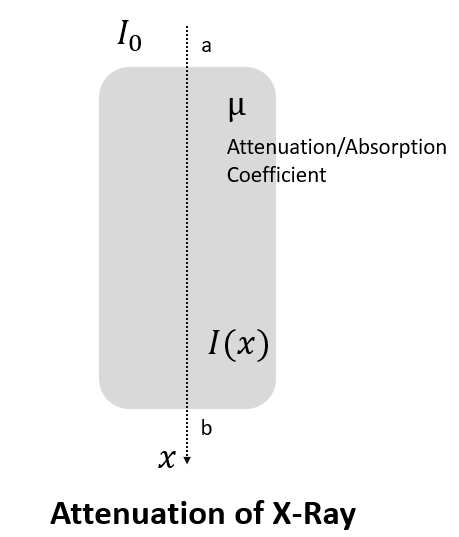
\includegraphics[width=0.4\textwidth]{img/background_img/attenutation}
	\caption{Attenuation}
	\label{fig:attenutation}
\end{figure}

\subsubsection{Hounsfield Units}
Hounsfield units (HU) represents the average attenuation value of each voxel compared to the attenuation value of water. CT numbers can take value between -1000 and 1000 while 2000 shades of grey is out of the capacity of human eyes can distinguish. Thus, only a limited number of HU are displayed for human interpretation. Lung window is normally set to [-1250, 250]. Figure \ref{fig:HU_value} shows some common HU value range of different matters.
\begin{figure}[h]
	\centering
	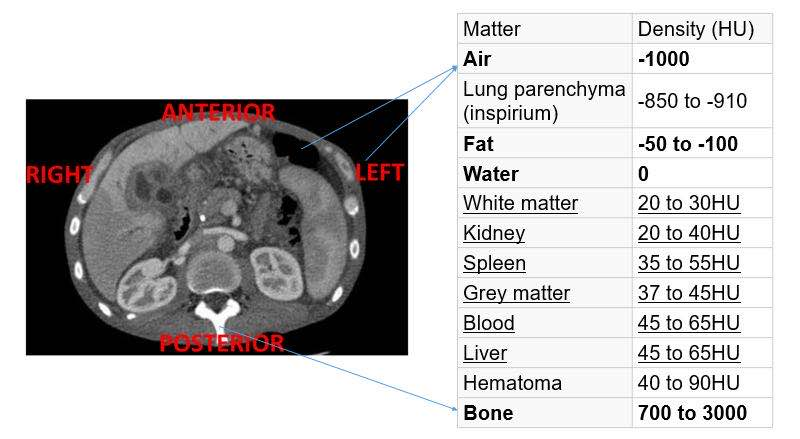
\includegraphics[width=0.8\textwidth]{img/background_img/HU_value.png}
	\caption{Common Hounsfield Unit values including human body tissue}
	\label{fig:HU_value}
\end{figure}

\subsection{Thick and thin slices}
Thin slices are generally regarded as planes representing thickness of less than 3mm \footnote{http://tech.snmjournals.org/content/36/2/57} In our work, we experienced slice thickness from 1mm to 8mm. \\
{\color{red} In medical CT scanning, considering the dose of CT, and the equipment limitation, thick slice tend to show little or no slice-wise information along the axial slices.} An illustration of thick and thin slice difference is shown in figure \ref{fig:thick_thin_slice}

\begin{figure}[h]
	\centering
	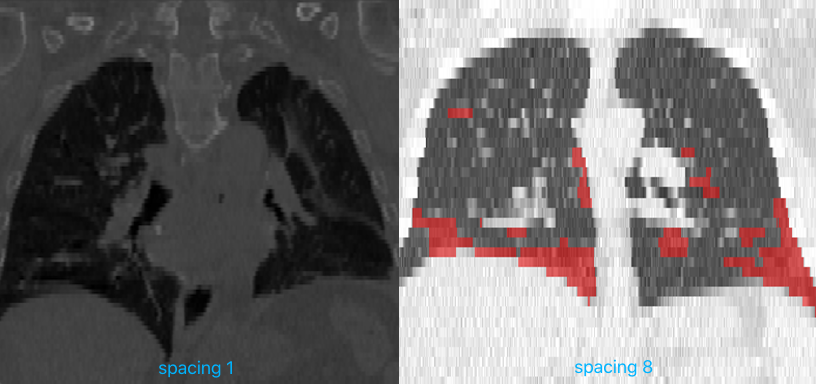
\includegraphics[width=0.8\textwidth]{img/background_img/thin_thick_slice.png}
	\caption{Spacing diversity along the Z (Axial) axis. Left: thin slice with spacing 1; Right: thick slice with spacing 8.}
	\label{fig:thick_thin_slice}
\end{figure}
\newpage

\section{Deep learning fundamentals}
In this section, we briefly mention some of the fundamentals of Deep Learning and some layer structures used in our experiment, note that most of our notation follows the book \textit{Deep Learning}\cite{Goodfellow-et-al-2016}.

\subsection{Optimization in training neural network}
%TODO mention optimizers here
\subsubsection{Gradient Descent}
Fist of all, Gradient Descent Algorithm leverages the first order derivative to modify the weights so that a function gradually reach its local minima. The mathematical definition is:
$$\boldsymbol{\theta}=\boldsymbol{\theta}-\boldsymbol{\alpha} \cdot \nabla \mathrm{J}(\boldsymbol{\theta})$$ 
in which $\mathrm{J}$ denotes the loss function, $\theta$ is the trainable parameter and $\alpha$ is the learning rate. 
\subsubsection{Adam optimizer}

%TODO adam optimization
\subsection{Convolutional Neural Network}
%TODO provide a brief theoretical summary of Convolution here
Convolutional neural networks (CNN) improved deep learning with respect to \textbf{Sparse interactions, parameter sharing and equivariant representations} that employ mathematical convolution operation denoted with asterisk symbol $*$. The imaging domain usually make use of discrete convolution: $$s(t)=(x * w)(t)=\sum_{a=-\infty}^{\infty} x(a) w(t-a)$$
We here clarify that in our following notation, we call $x$ the \textbf{input}, $w$ \textbf{kernel} or \textbf{weight}, and $s$ \textbf{output} or \textbf{feature map}.\\
In two dimensional case:
$$S(i, j)=(I * K)(i, j)=\sum_{m} \sum_{n} I(m, n) K(i-m, j-n)$$
\subsection{Activation function}
Activation function $\phi$ (usually non-linear) introduce non-linearity into neural networks.
In modern Neural Networks, some of the activation functions are:
\begin{itemize}
	\item Recitified Linear Unit (RelU): $\sigma(x)=\max (0, x)$
	\item Eponential Linear Unit (Elu): $\sigma(x)=\left\{\begin{array}{ll}\alpha\left(e^{x}-1\right) & \text { for } x<0 \\ x & \text { for } x \geq 0\end{array} \mid \alpha \geq 0\right.$
	\item Leaky Relu: $\sigma(x)=\left\{\begin{array}{ll}0.01 x & \text { for } x<0 \\ x & \text { for } x \geq 0\end{array}\right.$
	\item Sigmoid: $\sigma(x)=\frac{1}{1+e^{-x}}$
	\item Softmax: $\sigma(\boldsymbol{x})_{i}=\frac{e^{x_{i}}}{\sum_{j=1}^{n} e^{x_{j}}} \mid i \in\{1, \ldots, n\}$ Softmax scale the layer output between 0 and 1 and its sum = 1.
\end{itemize}

\begin{figure}[h]
	\centering
	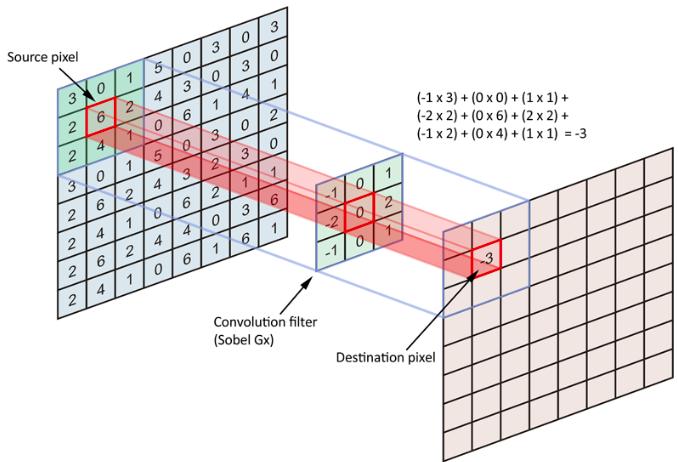
\includegraphics[width=0.8\textwidth]{img/background_img/convolution}
	\caption{An example of convolution using Sobel filter} 
	%TODO change citation \footnote{https://medium.com/pallawi.ds/ai-starter-build-your-first-convolution-neural-network-in-keras-from-scratch-to-perform-a059eaa6d4ff}
	\label{fig:convolution}
\end{figure}

\subsection{Pooling}
Pooling function modify the output of a layer at a specific location through summarizing its neighboring outputs that helps an approximate invariant. Max pooling is simply the maximum output within a neighborhood. Average pooling takes the average of the neighborhood as output instead of the maximum. An illustration of pooling is shown in figure \ref{fig:pooling}
\footnote{https://link.springer.com/article/10.1007/s00521-019-04296-5/figures/1}
\begin{figure}[h]
	\centering
	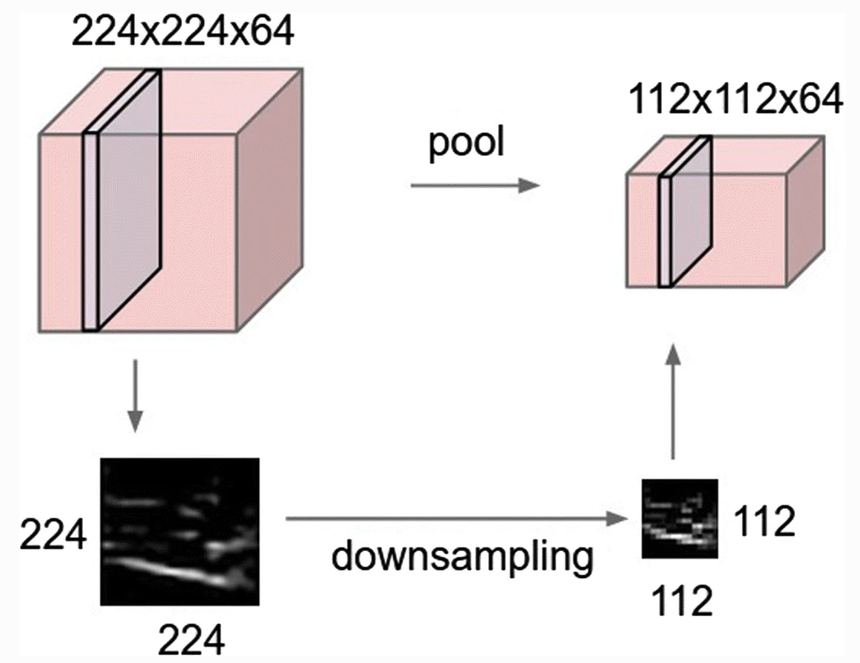
\includegraphics[width=0.6\textwidth]{img/background_img/pooling_img}
	\caption{Downsampling using pooling}
	\label{fig:pooling}
\end{figure}

\subsection{Batch Normalization}
Batch normalization (BN) was proposed in \cite{BatchNorm} to mitigate \textbf{internal covariate shift} by fixing the mean and variance of each layer's inputs so that it allows each layer of the network to learn more independently from the rest of the layers.\\

Batch Normalization adds two trainable parameters to each of the layer. The process of BN is shown below:
\begin{algorithm}
    \caption{Batch Normalisation}\label{BatchNorm}
    \hspace*{\algorithmicindent} \textbf{Input:} Values x over a mini-batch: $Batch = {x_{1...m}}$, $\gamma$, $\beta$\\
    \hspace*{\algorithmicindent} \textbf{Output:} $BN_{\gamma,\beta}(x_{1...m})$
    \begin{algorithmic}[]
    \State $\mu_{\mathcal{B}} \gets \frac{1}{m} \sum_{i=1}^{m} x_{i}$    
    \State $\sigma_{\mathcal{B}}^{2} \leftarrow \frac{1}{m} \sum_{i=1}^{m}\left(x_{i}-\mu_{\mathcal{B}}\right)^{2}$
    \State \Comment{Normalizing}
    \State $\widehat{x}_{i} \leftarrow \frac{x_{i}-\mu_{\mathcal{B}}}{\sqrt{\sigma_{\mathcal{B}}^{2}+\epsilon}}$  
    \State \Comment{Scale and shift}
    \State $y_{i} \leftarrow \gamma \widehat{x}_{i}+\beta \equiv \mathrm{B} \mathrm{N}_{\gamma, \beta}\left(x_{i}\right)$
    \end{algorithmic}
    \end{algorithm}

%TODO add more bullshit about batch normalization

\subsection{Attention Gate}
%TODO add details of the impelemted attention gate to the network
Attention Gate proposed in \cite{Attention_gate_network} provided a way that we can train the network for segmentation with extra localization objective.
Let $\mathbf{x}^{l}=\left\{\mathbf{x}_{i}^{l}\right\}_{i=1}^{n}$ denotes the activation map over a layer such that $x_{i}^{l}$ is the pixel-wise feature vector with dimension equals to the number of feature maps of the output. Attention Gate learn a scaling vector $\alpha_{i}^{l}$ as the weight to scale the feature vector, more formally:
$$\hat{\mathbf{x}}^{l}=\left\{\alpha_{i}^{l} \mathbf{x}_{i}^{l}\right\}_{i=1}^{n}$$
The additive attention in the paper, can then be written as:
$$q_{a t t, i}^{l}=\psi^{T}\left(\sigma_{1}\left(\boldsymbol{W}_{x}^{T} \boldsymbol{x}_{i}^{l}+\boldsymbol{W}_{g}^{T} \boldsymbol{g}+\boldsymbol{b}_{x g}\right)\right)+b_{\psi}$$
$$\alpha^{l}=\sigma_{2}\left(q_{a t t}^{l}\left(\boldsymbol{x}^{l}, \boldsymbol{g} ; \boldsymbol{\Theta}_{a t t}\right)\right)$$
in which $\sigma_{1}$ denotes a non-linear activation function such as ReLU and $\sigma_{2}$ is a normalizing function so that $\sum_{i} e^{q_{a t t, i}^{l}} = 1$. In the paper, the author used sigmoid as activation function. Note the the attention gate is usually obtained from a coarser feature map. Figure \ref{fig:att_gate} shows the attention gate structure.

\begin{figure}
\centering
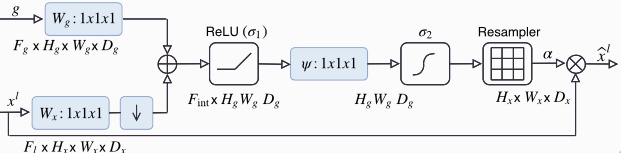
\includegraphics[width = 0.8\textwidth]{img/background_img/attention_gate}
\caption{Attention Gate structure proposed in \cite{Attention_gate_network}}
\label{fig:att_gate}
\end{figure}


\subsection{Encoder-Decoder architecture}
One of the breakthrough in both medical and non-medical segmentation is the presense of an Encoder-Decoder architecture network. Encoder combines non-linear feature extracting with convolution and down-sampling so that the Encoder can learn a rather 'rich hidden space representation'. The Decoder generates segmentation through upsamle or transpose convolution so that the network ouput is the same dimension of the input images. Paper \cite{Liu2018DeepCN} leveraged the Encoder-Decoder to segment bones in MR images. Figure \ref{fig:segnet_encoderdecoder} shows the encoder-decoder architecture leveraged in the paper.

\begin{figure}
\centering
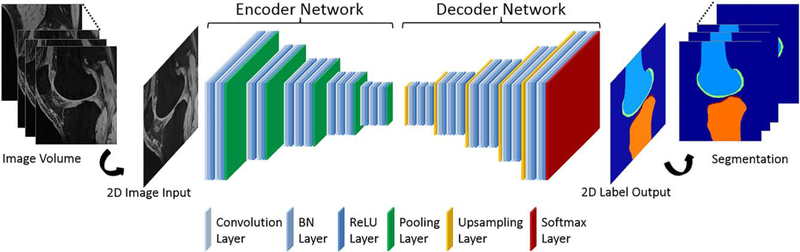
\includegraphics[width = 0.9\textwidth]{img/background_img/segnet_background}
\caption{An Encoder-Decoder structure network proposed in \cite{Liu2018DeepCN}}
\label{fig:segnet_encoderdecoder}
\end{figure}


\subsection{U-Net and skip connections}
This section we introduce several well known methods in medical segmentation. Unet \cite{ronneberger_u-net_2015} and its variations plays a dominant role in current medical segmentation tasks, and it is often used as a baseline model for performance evaluation in the literature.\\

U-Net \cite{ronneberger_u-net_2015} is among one of the most widely used medical segmentation models since the day it was proposed based on the Encoder-Decoder network structure it proposed. The original Unet consists of a contracting path followed by an expansive path that gives a "U" shaped architecture. The network architecture is shown in figure \ref{fig:unet-arch}.
Later this 2D model was extended to 3D version in \cite{ourselin_3d_2016} for for Kidney segmentation tasks so that the model learn features from information implicated between slices.\\
\begin{figure}
\centering
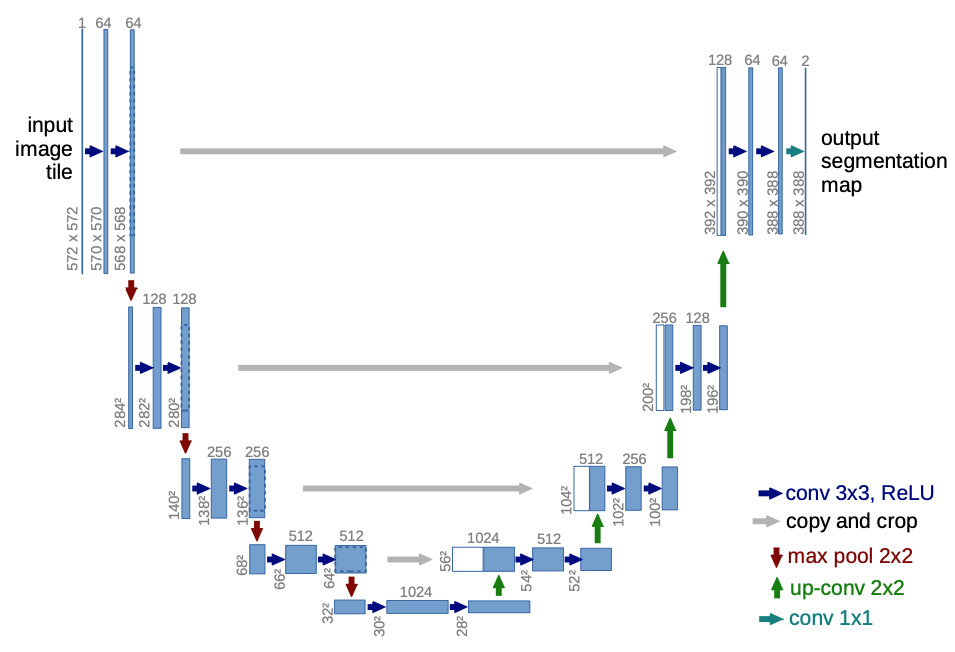
\includegraphics[width = 0.8\textwidth]{img/Unet_architecture}
\caption{Original Unet architecture in \cite{ronneberger_u-net_2015}}
\label{fig:unet-arch}
\end{figure}

VNet \cite{milletari_v-net_2016} is another 3D variation of Unet, and the network performed evaluation on prostate dataset. Each block of convolution has a residual feature that the input of the block is added to the last convolutional layer. The author argued that leverage residual structure enables network convergence in a fraction of the amount of time other network used.


\section{Small Sample Segmentation}

\subsection{Data augmentation}
In medical domain, huge dataset consists of large numbers of carefully labelled samples is rarely available due to heavy workload for annotations, rarity of disease, ethic issues of data acquire process and data privacy. Furthermore, different data acquire protocols (i.e. CT machines used by different hospitals) brings difficulties to clinical practice for good accuracy of existing pre-trained models. As a result, few shot learning and/or few shot segmentation has been explored in recent years. 
In this section, we focus on a few approaches that has been used in current literature which aim to explore the potential of existing training samples through various augmentation methods to alleviate the insufficient training samples in medical imaging. We discuss data augmentation method as well as the amount of data used in each work. Table \ref{tab:Augtable} provide an overview of each method.

\subsection{Traditional Data Augmentation}
Traditional Data augmentation methods in imaging domain refers to the process that does not require such training data to learn a transformation.\\

Paper \cite{zhang_when_2019} investigated data augmentation methods under 3D medical domain of MR and ultrasound images. 
The data augmentation process consists of a sequence of traditional transformation techniques. The paper argued that sharpness in medical images during training process limits model generalization thus applying gaussian filter to images take noise into consideration. Brightness and contrast difference caused by variations in scanning protocols brings potential domain shift thus a sequenced random shift followed gamma correction and random linear transform in intensity are reasonable data augmentation methods. Finally spatial transformations including rotation, flipping, scaling and deformation is added to the augmentation process.

The source domain in this method is Prostate dataset \footnote{http://medicaldecathlon.com/index.html\#tasks} which consists 48 4D volumes.
We argue here that the stacked transformation is a physical transformation process independent to the size of dataset because no learning or training process is required in this augmentation method thus might bring benefits to our task. However, although Deep learning models (Convolutional Neural Networks) are scale and rotation invariant, medical images differs from natrual images that scanning was conducted with a certain position, i.e. patients usually lie on a CT bed facing up for CT scanning. Thus flipping the lung volumes or rotating the lungs more than 5 degrees is less reasonble.\\


%%%---------
Another method "mixup" by \cite{zhang_mixup_2018} based on generic vicinal distribution, which generates new samples through interpolation between two existing data. The author argued that this method works as a regularizer which encourages linear behavior between training samples. In terms of imaging, the augmentation is applied to CIFAR 10 (2D non medical) Dataset. The calculation method in paper follows the following equations where $x_{i}$ and $x_{j}$ are training examples and $\lambda$ is usually sampled from beta distribution.
$$\tilde{x}=\lambda x_{i}+(1-\lambda) x_{j}$$
$$\tilde{y}=\lambda y_{i}+(1-\lambda) y_{j}$$
The work was originally implemented on training GANs. Later in medical domain, \cite{panfilov_improving_2019} further investigated mixup method on Knee MR images on OIA database \footnote{http://www.oai.ucsf/.edu/} that consists of 88 3D MRI scans. The work showed mixup improves generalization under their experiment setup while having risk of slight underfitting due to to the strong regularization. The author further mentioned not using weight decay in the experiment solve the underfitting issue.
\cite{tajbakhsh_embracing_2020} summarized mixup augmentation method gives "soft labels". Variations of the mixup method utilize asymmetric is further explored in \cite{li_overfitting_2019} trained on Brain MR images, and the method reports huge gain under their experiment setup.

\subsection{Learning for augmentation}
Following the traditional augmentation methods, we here want to discuss a few medical image augmentation based on deep learning. Specifically we focus on those who used one or a few data during the augmentation so that it follows the small sample segmentation setup.\\

%TODO citation in adversarial defense
Adversarial defense was deployed in \cite{suk_brain_2019} for the augmentation of small samples in Brain MR segmentation. Adversarial samples generated though Fast Gradient Sign Method\cite{goodfellow_explaining_2015} and then added as training data to improve the robustness. Paper in \cite{chen_one-shot_2020} leverage paired MRI-CT data to construct a cycle-GAN model that convert an given MRI to a CT style image to segment Craniomaxillofacial Bone structure.\\

\begin{table}
\begin{tabular}{lllll}
\hline
Paper                                             & Method                        & Dataset              & Number of samples &  \\
\hline
\cite{zhang_when_2019}       & Stacked traditional transform & Prostate dataset     & 48 4D volumes     &  \\
\cite{zhang_mixup_2018}       & mixup                         & CIFAR 10             & Huge              &  \\
\cite{panfilov_improving_2019} & mixup                         & Knee MR images       & 88 3D MRI         &  \\
\cite{li_overfitting_2019}   & Asymmetric mixup              & BraTS               &  not specified             &  \\
\cite{suk_brain_2019}                    & Adversarial defense           & MRBrainS18 challenge & 7 train, 14 test  &  \\
\cite{chen_one-shot_2020} &  Cycle GAN &  Brain CT and MR&1 MRI-CT pair; Large MRI\\
\hline
\end{tabular}
\caption{Data Augmentation methods}
\label{tab:Augtable}
\end{table}

\subsection{Transfer Learning}
In medical domain, few shot learning mainly focus on transfer learning from pre-trained networks that leverage both medical and non-medical datasets.\\

%Although recent machine learning community have seen a growing number of medical segmentation public dataset available, the amount of data samples is still less desirable compared to natural, non-medical datasets. Thus researchers have seek for methods that leverage natural images.\\

In Lung CT segmentation area, Sports-1M dataset has been used as source domain to train a multi-task learning model for nodule malignancy prediction and rating \cite{hussein_risk_2017}. The author reported significant improvement in the prediction accuracy, however, did not mention the proportion of data used for transfer training.\\

People tend to choose datasets from closer domain for transfer learning. It is reasonable to consider methods that transfer across disease in the same structure under the same modality. In our case, we might want to investigate transfer learning from NSCLC Dataset to Covid segmentation set given that both of them are lung CT scans.\\

Recent work explored several across disease transfer learning training techniques under MRI domain \cite{wang_improving_2019}. The paper evaluated three transfer learning methods trained on 3D U-Net by Fine tuning the last three layers, Fine tuning the decoder and Fine tuning all model parameters. 
The Source Dataset: Multiple Sclerosis Dataset consists 3630 MRI volumes and used Brain Tumor Dataset as Target dataset including 210 high-grade glioma (HGG) and 75 low-grade glioma (LGG) Brain MRI scans. The training target is a decaying weighted categorical cross entropy loss weighted by relative voxel. Their best validation performance of pre-trained network achieved validation performance AUC 0.77. Experiment result on 20, 50, 100 and 150 samples during Fine tuning respectively showed that Fine tuning all parameters out performed the rest methods in most cases.\\

One potential drawback is that compared to the our task, the target training set is relatively larger, the performance is expected to be less ideal when using "fine tune all" method using 4 or less volumes in our case.

\subsection{Special network design}
Transfer learning methods usually require small samples to update millions of parameters that take the risk of overfitting \cite{shaban_one-shot_2017}. The design of multiple branch network, usually includes conditioner arm and segmentation arms inspired the deep learning in medical domain to go beyond transfer learning while encourage a stronger between-arms interaction to compensate the lacking in pre-trained model \cite{roy_squeeze_2019}. The proposed method perform 3D volume segmentation at test time while use 2D images during training. However the method requires start and end slice to be indicated for each query volume and still not achieving good dice score.\\

Paper \cite{suk_brain_2019} trained segmentation of Brain MR image on 7 brain volumes after Adversarial defense augmentation. The work first split the segmentation from easy to hard into 2 individual classifiers then joint learning with dense pixel segmentation. The author reported that the result outperformed Unet and Vnet method trained from scratch. We argue that the augmentation provide good result in the segmentation accuracy while the segmentation part is not well explained in the paper. We have emailed the author for further details.

% TODO change citation in table header
\begin{table}
\begin{tabular}{p{1cm} p{5cm} p{4cm} p{4cm}}
\hline
Paper    & Method                                & Domain Details                                          & Task                                       \\
\hline
{\cite{shaban_one-shot_2017}} & Design Conditional Branch             & Target PASCAL-5        & Few shot segmentation                      \\
{\cite{rakelly_few-shot_nodate}} & Guidance network                      & Target PASCAL VOC             & Few shot segmentation                      \\
{\cite{hussein_risk_2017}} & Non medical to medical transfer       & Source: Sports-1M;  Target: Lung nodule                  & Multi-task learning: prediction and rating \\
{\cite{wang_improving_2019}} & Across domain transfer                & Source: MSD; Target: Brain Tumor Dataset & Segmentation                               \\
{\cite{shaban_one-shot_2017}} & Augmentation+pixel dense segmentation & Only trained on 7 brain Volumes                         & Dense segmentation                         \\
{\cite{suk_brain_2019}}  & Branch network design                 & --                                                      & Segmentation                               \\
\hline
\end{tabular}
\caption{Small sample methods in medical and non-medical domain}
\label{tab:small sample learning}
\end{table}	

\subsection{Learning with unlabelled data}
Another common scenario with medical imaging is that, a small set of labelled annotations is available and a relatively larger set of data was collected but not labelled. In this section, we briefly mention three types of work that leverage unlabelled data: training encoder, noise removing, and semi-supervise learning. Both training encoder and noise removing serves as a pretrained network that are usually fined-tuned using the methods we described in the previous section. Semi-supervise learning was proposed to further make use of the unlabeled samples to guide the network update more directly throughout the training process.

\subsubsection{Training encoder as initialization}
Training encoder part without expert labeling usually make use of spatial information of the image such as slice order \cite{10.1007/978-3-319-66179-7_47} and direction \cite{8759553}. \\

In the work \cite{8759553}, authors trained a network to predict a transformation of orientation by rotating or flipping the input slice, and then fine tune the network to classify retinal imaged of diabetes patients. One potential use of this type of initialzation for segmentation task is that we can append the Up-Convolution then transfer on segmentation labels.\\

Paper \cite{10.1007/978-3-319-66179-7_47} trained a encoder that, given a reference slice and a prediction slice, predict the prediction slice is above of behind the reference slide so that the network can learn spatial information using the unlabelled images.\\

\subsubsection{Noise removing}
Instead of training a surrogate task such as training encoder leveraging spatial or location information as a pretraining task, Zongwei Zhou \cite{zhou_models_2019} provided another probability for pretraining both encoder and decoder that used together can serve as weight initialization for a segmentation model, and encoder used on its own is a pretrained feauture extractor for classification task.\\

The work trained a Unet-style network that given a randomly cropped and sliced image, first destroy the image through a sequence of random non-linear transformation, local shifting, out/in-painting then forward the image to restore the original image by minimizing the mean-square-error during training. The author argue that in that way, both the generalizability and the detail feature encoding can be learnt which can be leveraged in later transfer learning process. Figure \ref{fig:genesis-net} showed the restoration process. The model was trained on Lung CT images which is close to our task while the provided model was in 3D version, later in the experiment stage, we actually flattened the pretrained weight into 2D for future training.

\begin{figure}
	\centering
	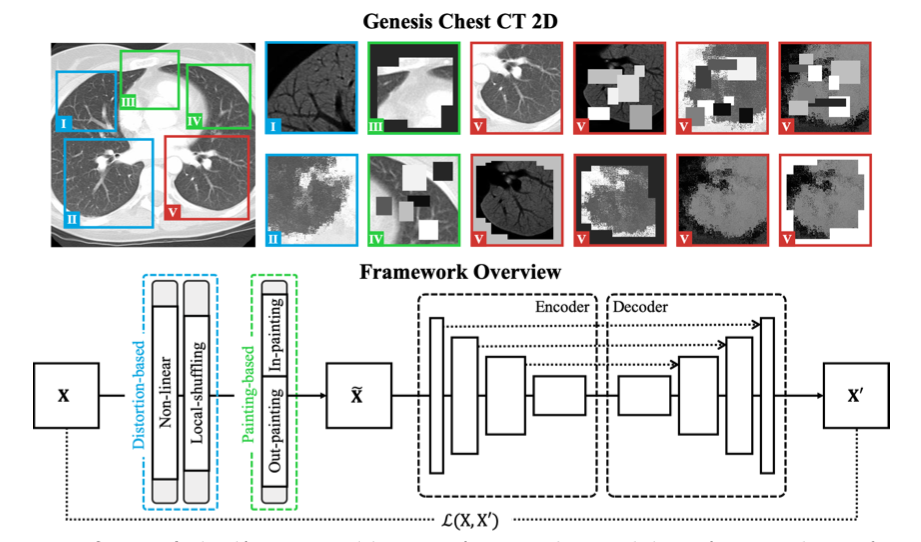
\includegraphics[width=0.8\textwidth]{img/background_img/Genesis_illustration.png}
	\caption{An illustration of Model Genesis pre-training (Figure from the original paper \cite{zhou_models_2019})}
	\label{fig:genesis-net}
\end{figure}

\subsubsection{Semi-supervise}
Semi supervise approach usually add a prediction consistency loss during training. \cite{tarvainen_mean_2018} propsed a teacher-student training strategt such that two networks are train together. The proposed so called 'Mean-teacher' network trained two network simultaneusly. The network design consists of two isomorphic networks that serves as teacher and student. In the beginning of the semi-supervise training, a copy of the teacher model is also created called the student network. For expert-labelled samples, the student model was update using the prediction loss.
Now given a new set of unlabelled raw images, the student network are trained using the prediction consistency cost between student and teacher model. The teacher model weights are updated periodically using an exponential moving average of the student network instead of back propogate the loss directly. Figure \ref{fig:mean-teacher} explains the training process. \\

We here further gives the defnition in the original work \cite{tarvainen_mean_2018}. More formally, define the consistency of the prediction as:
$$J(\theta)=\mathbb{E}_{x, \eta^{\prime}, \eta}\left[\left\|f\left(x, \theta^{\prime}, \eta^{\prime}\right)-f(x, \theta, \eta)\right\|^{2}\right]$$
where x is the input data (image), $\theta, \eta$ denotes the weight and noise in the teacher model and $\theta', \eta'$ denotes the weight and noise in the student model.
The weight update in the teacher model can then be written as:
$$\theta_{t}^{\prime}=\alpha \theta_{t-1}^{\prime}+(1-\alpha) \theta_{t}$$ in which $\alpha$ is the smoothing parameter showing how much the teacher want to move given the new student network.\\

\begin{figure}
	\centering
	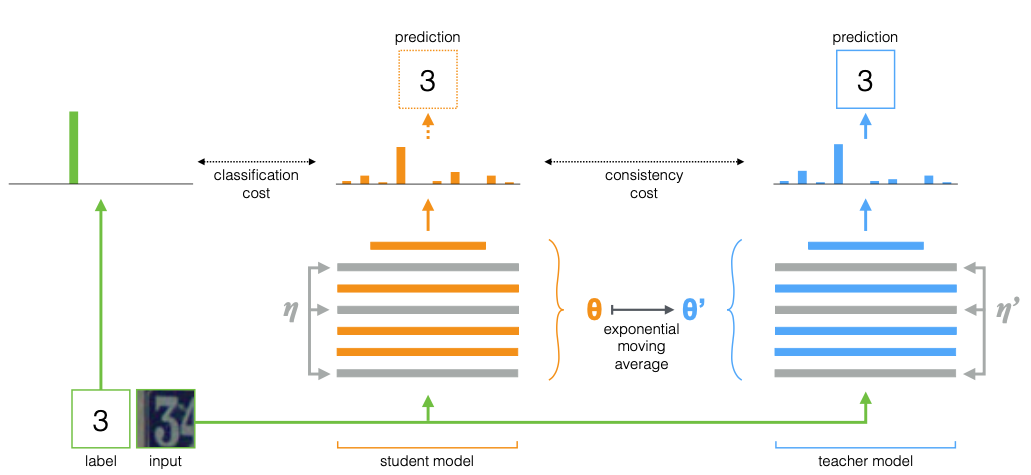
\includegraphics[width=0.8\textwidth]{img/background_img/mean-teacher.png}
	\caption{An illustration of mean teacher for semi-supervise learning (Figure from the original paper \cite{tarvainen_mean_2018})}
	\label{fig:mean-teacher}
\end{figure}

We argue here that this training strategy can help our task 2 given a relatively larger amount of unlabelled samples are available.

\section{Evaluation}
\subsection{Quantifying Segmentation prediction}
Loss function or objective function is a crutial component in neural network training. Segmentation tasks usually make use of \textit{Distribution loss}, \textit{Region based loss} and \textit{boundary-based} loss for training and evaluation of segmentation performance. Recent work in \cite{ma_segmentation_2020} summarized some common loss functions for segmentation. \\

\textbf{Cross entropy} (CE) measures the dissimilarity between the learned distribution and target distribution. 
$$CE = -\frac{1}{N} \sum_{i=1}^{N} \sum_{c=1}^{C} w_{c} \cdot (y_{i}^{c} \log p_{i}^{c})$$ where $y_{i}^{c}$ indicates the prediction result (correct or wrong) and $p_{i}^{c}$ denotes the predicted probability of pixel i for class c, $w_{c}$ is now 1 for original cross entropy loss.

Unet \cite{ronneberger_u-net_2015} training extend the CE by adding weight $w_{c}$. A common example for weight measurement is through the inverse proportion of observed class frequency. This modification potentially deal with imbalance class which is very common in medical domain.\\

\textbf{Dice loss} is a region based loss function that learn to optimize the Dice Coefficient (D). Vnet \cite{milletari_v-net_2016} first brought the Dice loss into machine vision community to solve the problem of highly biased prediction towards dominant area (e.g background) in medical segmentation.
 $$D=\frac{2 \sum_{i}^{N} p_{i} g_{i}}{\sum_{i}^{N} p_{i}^{2}+\sum_{i}^{N} g_{i}^{2}}$$
 Assume we segment N samples, $p_{i}$ denotes the prediction volume and $g_{i}$ denotes the ground-truth volume.
Dice loss usually require the label to be one hot encoded during training. One benefit is that Dice loss does not requires class balance methods such as weighting method in CE loss.\\

\textbf{Hausdorff Distance loss}(HD) aims to minimize the boundary distance between prediction and ground-truth segmentation masks. Similar to Dice loss, it also alleviate the class imbalance issue during training. However,directly minimizing Hausdorff Distance is intractable while an approximation (HD Loss) through distance transform (gray-level intensities of points inside foreground regions are changed to show the distance to the closest boundary from each point \footnote{https://homepages.inf.ed.ac.uk/rbf/HIPR2/distance.htm}).
$$L_{H D_{D T}}=\frac{1}{N} \sum_{i=1}^{N}\left[\left(s_{i}-g_{i}\right) \cdot\left(d_{G i}^{2}+d_{S i}^{2}\right)\right]$$

Paper \cite{ma_segmentation_2020} proposed that so far none of the papers in the literature provide a comprehensive comparison of the loss functions for segmentation task. Selecting loss function is still based on empirical comparison. For example, \cite{DBLP:journals/corr/abs-1809-10486} used compound loss function that combined CE and Dice together as training objectives overall gives good performance compared to individual loss functions.

\subsection{Evaluating Transfer Learning}
Loss function quantifies the transfer learning prediction accuracy. We further want to understand the model behaviours. For example: How weights are updated during fine tuning? Is Pretraining compared to random initialization result in different weights such that the the latent space are apart from each other?\\

Singular Vector Canonical Correlation Analysis (SVCCA) \cite{raghu_svcca_2017} developed by Google Brain provide a method that compares the latent space of different models or different layers. The method is more quite simple while useful for comparing high dimensional latent features.\\

First let $l$ denotes the output of layer over a dataset $D$, The paper perform the following SVCCA steps:
\begin{itemize}
	\item Given two layers of output $l_{1}$, $l_{2}$ that represent the learnt subspace on the dataset, perform singular value decomposition then select the new subspace $l_{1}'$, $l_{2}'$ which preserve 99\% of the original variance.
	\item Perform Canonical Correlation Analysis on the two subspace $l_{1}'$, $l_{2}'$ so that the two new subspaces are as correlated as possible through transfomation. Each direction has a correlation $\rho_{i}$
	\item The correlation of two subspaces is the average of each output correlation $\rho_{l_{1}, l_{2}} = \frac{1}{N}\sum_{i=0}^{N} \rho_{i}$
\end{itemize}

SVCCA interprets the result of any two learnt subspace over a dataset. Later in work \cite{raghu_transfusion_2019}, the author utilized the method to understand the behavior of transfer learning in rather larger amounts of data on medical classification task.\\
\newpage

%%%%%%%%%%%%%%%%%%%%%%%%%%%%%%%%%%%%
\chapter{Data}

%\section{Data description}
%One of the most straightforward way to deal with the limit amount of available data is to leverage as much related Medical Data as possible. We thus investigated several public available dataset for Lung CT scans in addition to the Covid-CT dataset.
%
%\subsection{NSCLC Dataset}
%NSCLC Dataset contains 402 Lung CT scans, of which 78 cases are anotated with left lung, right lung and pleural effusion area. A sample annotation is shown in figure \ref{fig:NSCLC_example}
%\begin{figure}[h]
%	\centering
%	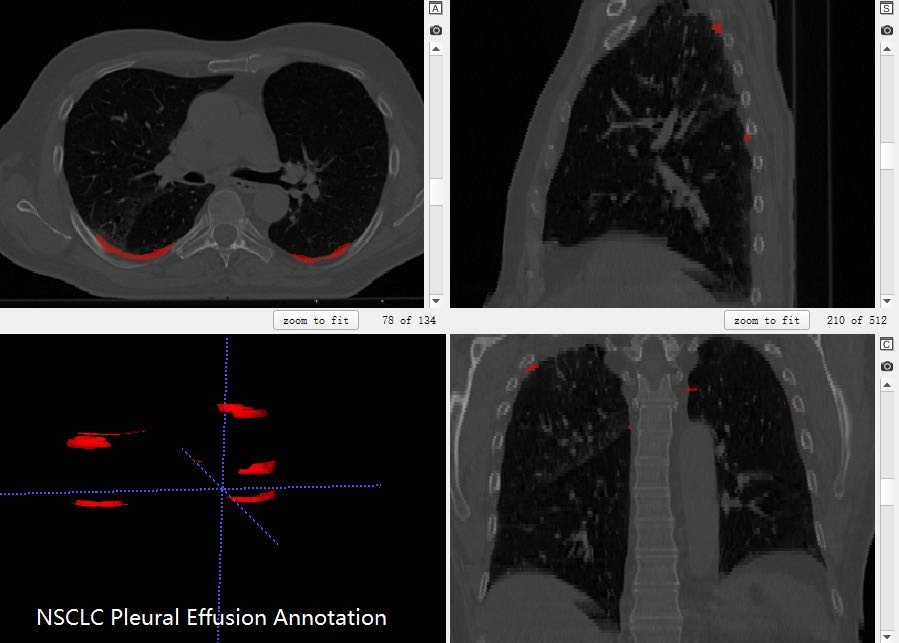
\includegraphics[width=0.6\textwidth]{img/Dataset/NSCLC}
%	\caption{An example volume from NSCLC Dataset with its annotation}
%	\label{fig:NSCLC_example}
%\end{figure}
%
%\subsection{MSD Lung Tumor}
%MSD Lung Tumor contains 63 Lung CT scans, annotating the Lung Cancer area. An example shown in figure \ref{fig:MSD_example}
%\begin{figure}[h]
%	\centering
%	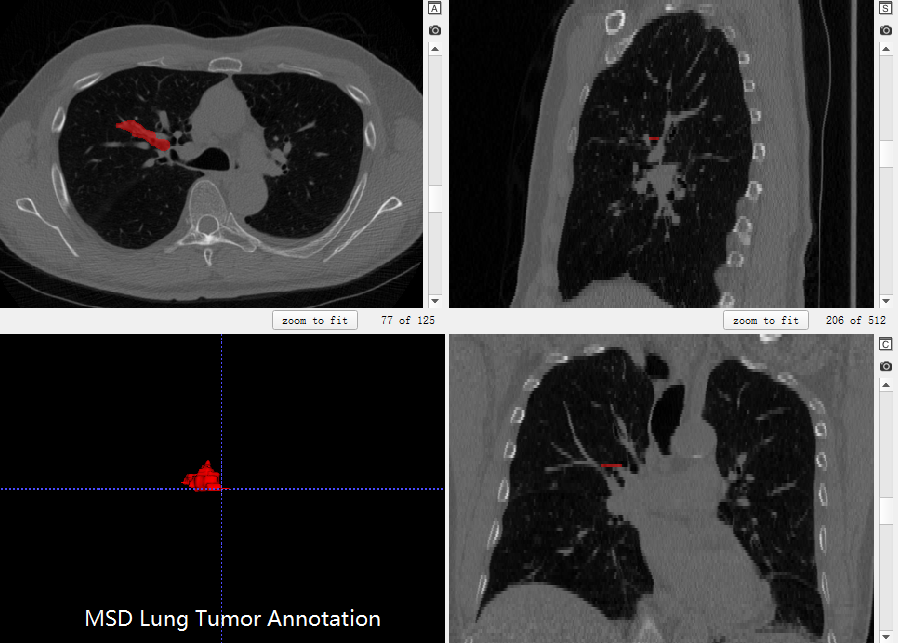
\includegraphics[width=0.6\textwidth]{img/Dataset/MSD}
%	\caption{An example volume from MSD Dataset with its annotation}
%	\label{fig:MSD_example}
%\end{figure}
%
%\subsection{MosMed Dataset}
%MosMed Dataset Contains 50 Annotated thick-slice Covid CT scans, as well as around 300 unannotated Lung CTs. We'd like to report here that we used only 200 unannotated slices because downloading keep giving me error due to location restriction. An example shown in figure \ref{fig:MosMed_example}
%\begin{figure}[h]
%	\centering
%	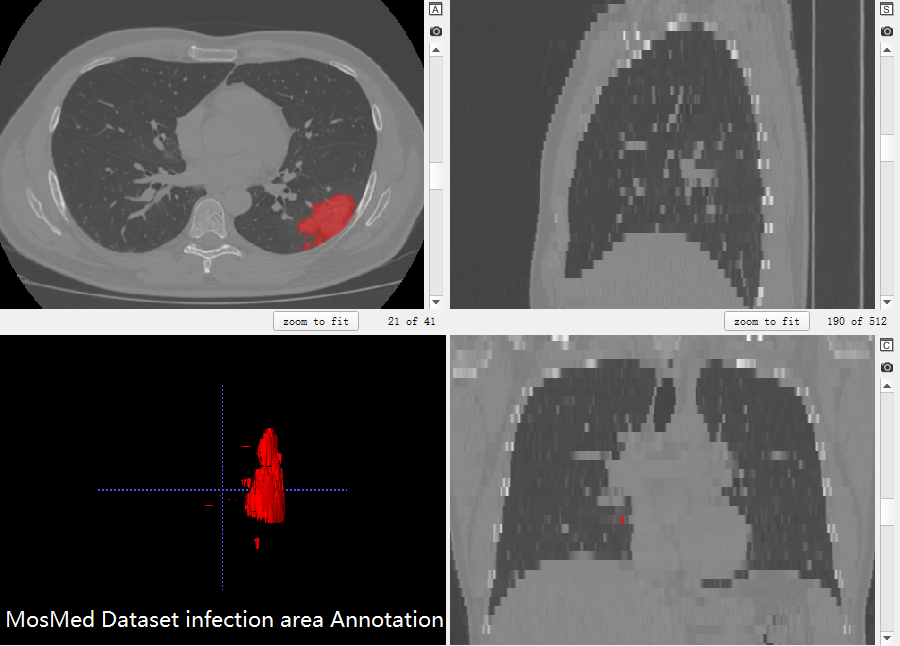
\includegraphics[width=0.6\textwidth]{img/Dataset/MosMed_example}
%	\caption{An example volume from MosMed Dataset with its annotation}
%	\label{fig:MosMed_example}
%\end{figure}
%
%
%\subsection{Covid Segmentation Benchmark}
%Covid Segmentation Benchmard contains 20 CT scans from 2 radiometric centers, of which 10 volumes thin-slice CT volumes and 10 thick slice CT volumes.
%\begin{figure}[h]
%	\centering
%	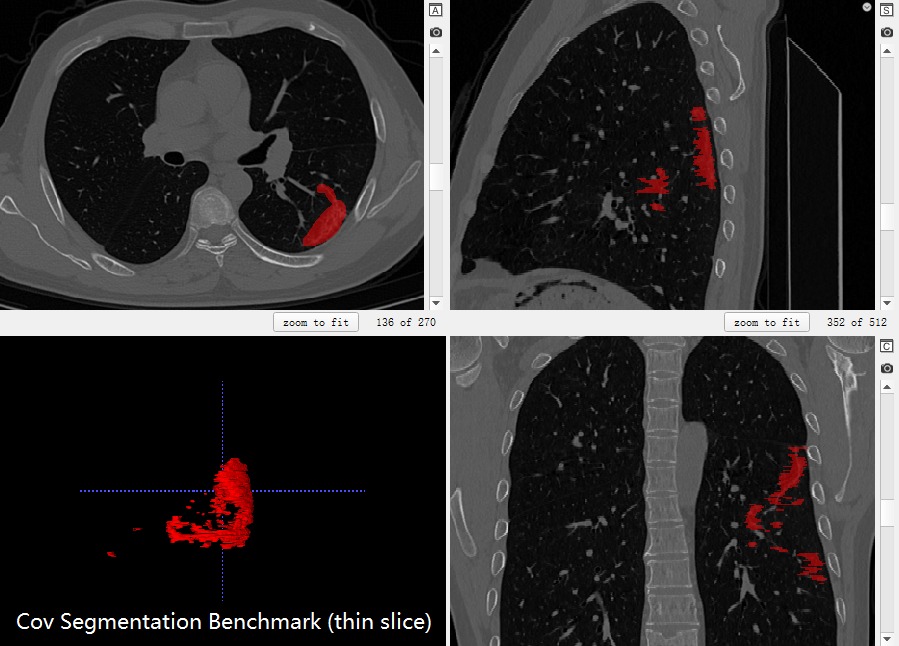
\includegraphics[width=0.6\textwidth]{img/Dataset/Cov_benchmark_thin}
%	\caption{An example volume from Cov Segmentation Benchmark (thin slice) with its annotation}
%	\label{fig:Covseg_thin}
%\end{figure}
%\begin{figure}[h]
%	\centering
%	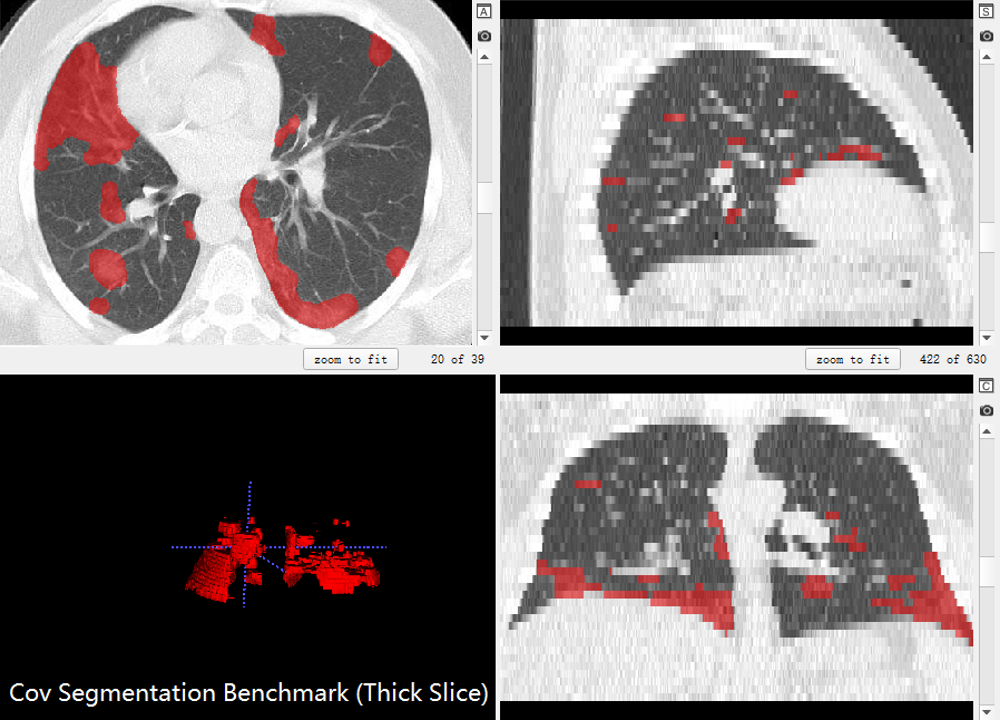
\includegraphics[width=0.6\textwidth]{img/Dataset/Cov_benchmark_thick}
%	\caption{An example volume from Cov Segmentation Benchmark (thick slice) with its annotation}
%	\label{fig:Covseg_thick}
%\end{figure}
%
%
%\section{Data preprocessing}
%The dataset used in this paper was collected from multiple centers with different equipment setup. Structseg2019, NSCLC, MSD Lung Tumor set are thin slice CT scans. MosMed contained 50 thick slice scans and the Covid segmentation benchmark are multi-center dataset from different centers. We argue that deep learning algorithms, especially segmentation tasks are sensitive to this difference. To make most use of the data, we first extract the lungs from the CT volumes. Then a sequence of preprocessing was performed including resampling, histogram equalization, and mean variance normalization. Most implementation used SimpleITK dataset
%
%\subsection{Processing into functional features}
%Lung CT scans images includes the lung tissue as well as bones and meshes that influence the preprocessing such as normalization as well as future segmentation. We intended to first segment the lung tissue out for better focus.\\
%\textbf{Lung segmentation using watershed algorithm}\\
%
%\textbf{Lung segmentation Using pre-trained Deep learning models}\\
%Deep learning method provide finer results when facing severe pathology. Work in \cite{hofmanninger_automatic_2020} provided a promising result for Lung segmentation. In addition, they further improve their lung segmentation model with Covid-19 Lung data.\\
%
%We leveraged their models provided in their github repository \footnote{https://github.com/JoHof/lungmask}. Original volumes from the Lung datasets went through the model, we threshold the lung out and set the uninterested area (background) as 0. Figure \ref{fig:filtered_Lung} showed and example lung volume before and after filtering the lung tissue.
%
%\begin{figure}[h]
%\centering
%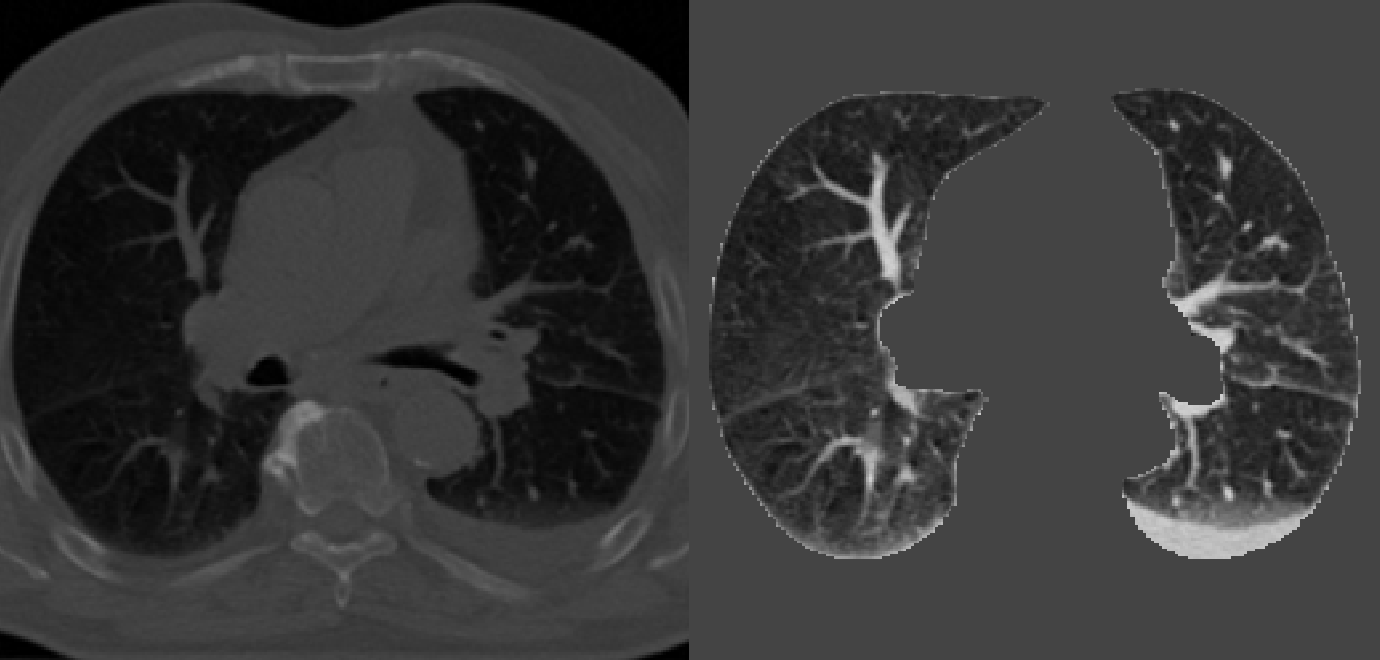
\includegraphics[width=0.5\textwidth]{/Users/tianyangsun/Desktop/Project/MSc-report/img/filtered_lung/nsclc_filteredlung_axial.png}
%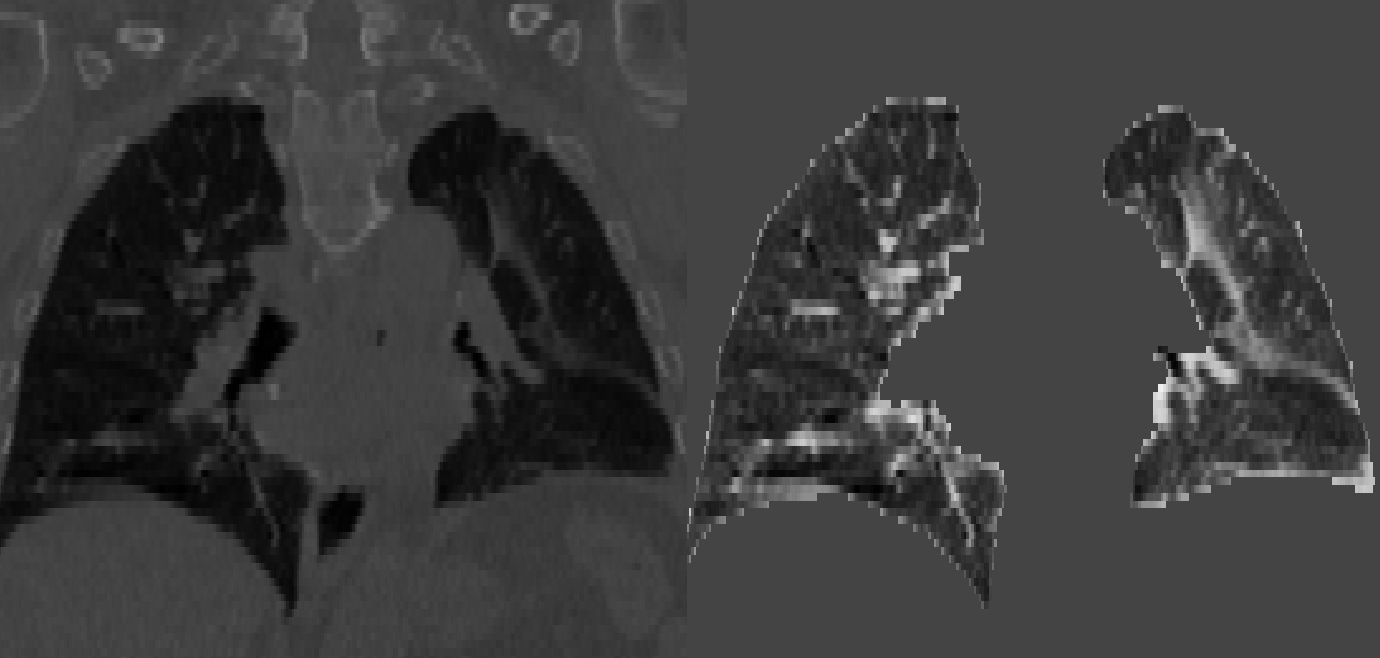
\includegraphics[width=0.5\textwidth]{img/filtered_lung/nsclc_filtered_coronal.png}
%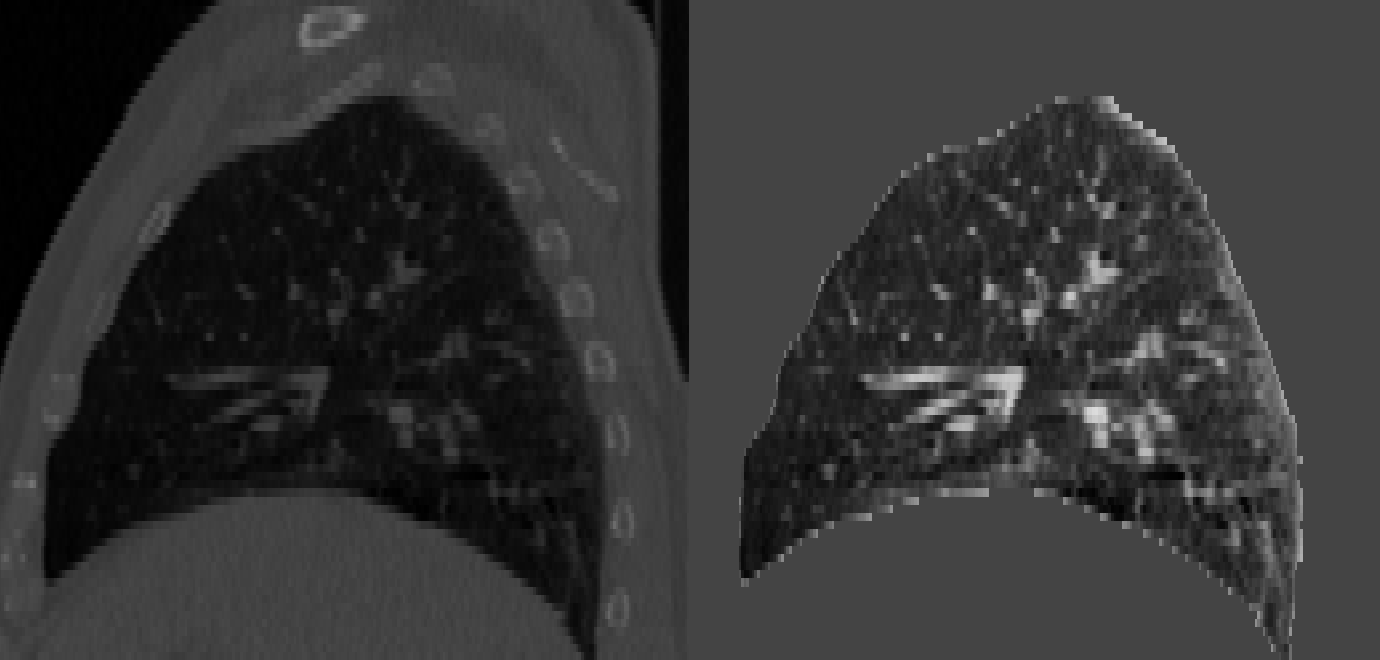
\includegraphics[width=0.5\textwidth]{/Users/tianyangsun/Desktop/Project/MSc-report/img/filtered_lung/nsclc_filteredlung_Saggital.png}
%\caption{An example from NSCLC Pleural Effusion dataset showing the volumes before and after lung filtering. (Top: Axial view, Middle: Coronal view, Bottom: Saggital View)}
%\label{fig:filtered_Lung}
%\end{figure}
%
%\subsection{Resampling}
%\begin{figure}[h]
%	\centering
%	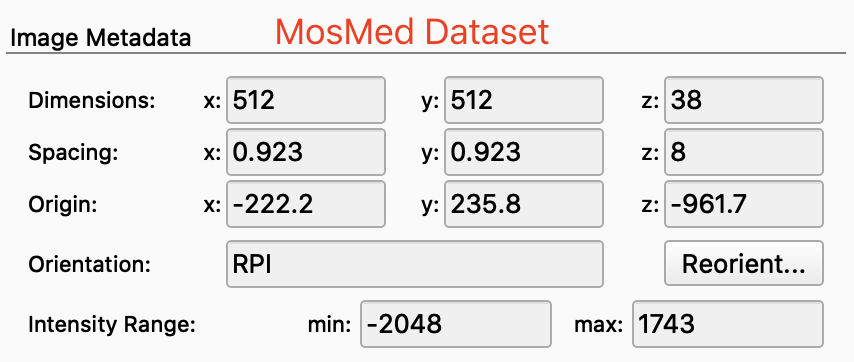
\includegraphics[width=0.5\textwidth]{/Users/tianyangsun/Desktop/Project/MSc-report/img/spacing_diverse/Mosmed_dataset.png}
%	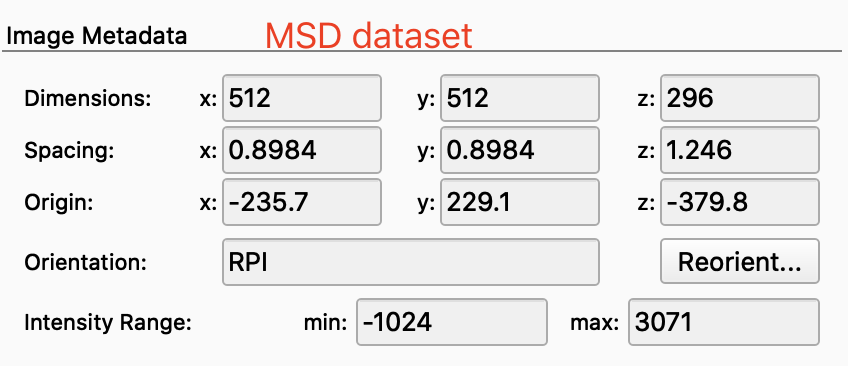
\includegraphics[width=0.5\textwidth]{/Users/tianyangsun/Desktop/Project/MSc-report/img/spacing_diverse/MSD_metadata.png}
%	\caption{An example of different spacing information from MosMed and MSD dataset}
%	\label{fig:Spacediverse}
%\end{figure}
%Figure \ref{fig:Spacediverse} showed the diveristy in spacing from different datsets. To deal with the different spacing for multi-domain data, we resampled the data to spacing (1, 1) in the Axial view and remain not changed in the Z axis.
%
%\subsection{Mean Variance Normalization}
%We performed Mean Variance Normalization (Z score normalization) for the lung tissue voxels by subtracting each volume with its mean and divided by its standard deviation. So that the data has zero mean and standard deviation of 1. 
%$$z=\frac{x-\mu}{\sigma}$$ of which $\mu$ is the mean and $\sigma$ is the variance. Figure \ref{fig:normalization} showed the intensity range before and after normalization
%
%\begin{figure}[h]
%	\centering
%	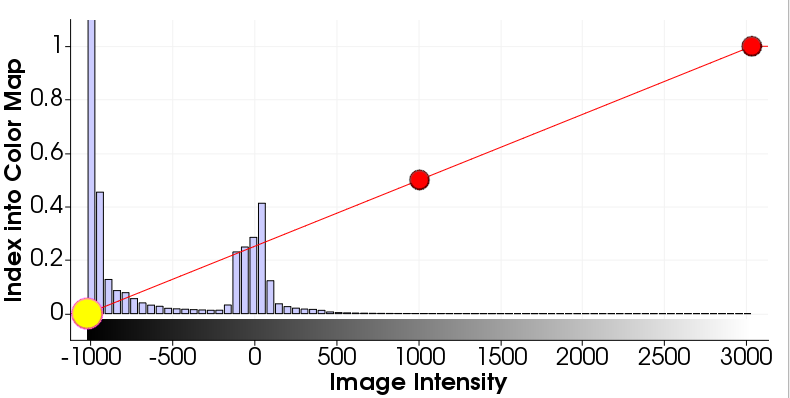
\includegraphics[width=0.5\textwidth]{/Users/tianyangsun/Desktop/Project/MSc-report/img/normalization/intensity_before.png}
%	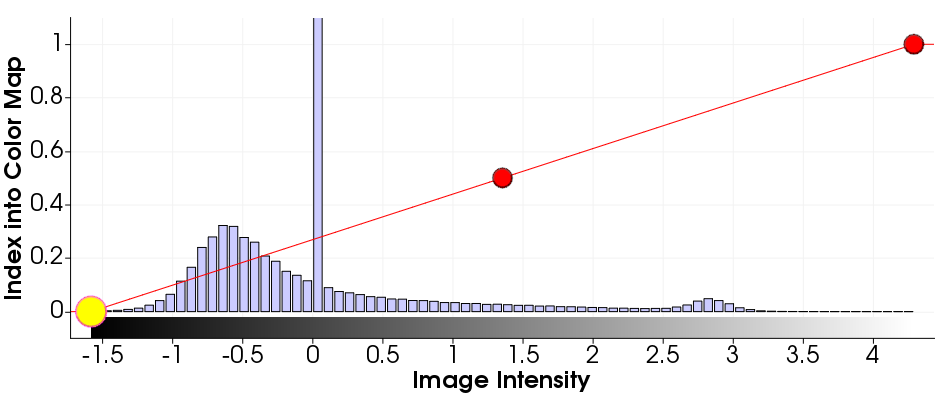
\includegraphics[width=0.5\textwidth]{/Users/tianyangsun/Desktop/Project/MSc-report/img/normalization/intensity_after.png}
%	\caption{An example showing the intensity range before and after normalization (Top: before normalization; Bottom: after normalization)}
%	\label{fig:normalization}
%\end{figure}
%
%\newpage
%\section{Data Augmentation}
%% TODO: add examples showing the transformation in augmentation
%For data augmentation, we investigated some of the augmentation techniques in medical imaging domain, each of the augmentation techniques was carefully chosen matching real medical situation.\\
%
%\textbf{Rotation:} We performed a small random rotation between [-3, 3] degree considering the pose variation when lying down on the scanner.\\
%%\begin{figure}[h]
%%	\centering
%%	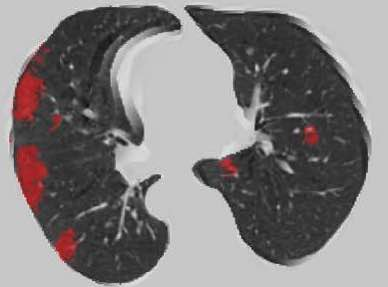
\includegraphics[width=0.4\textwidth]{img/augment/rotation}
%%	\caption{An example of rotation using MosMed Dataset}
%%\end{figure}
%
%\textbf{Elastic Transformation:} We performed a small elastic transformation considering lying down and holding breath when scanning Lung CT might brings shape change to the lungs tissue.\\
%%\begin{figure}[h]
%%	\centering
%%	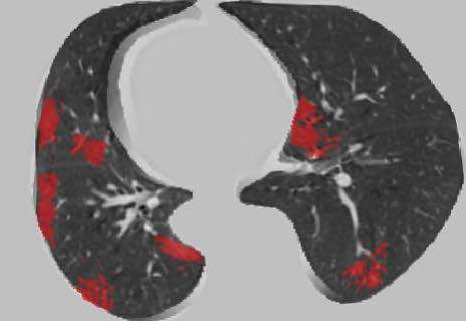
\includegraphics[width=0.4\textwidth]{img/augment/elastic_transformation}
%%	\caption{An example of elastic transformation using MosMed Dataset}
%%\end{figure}
%
%\textbf{Random Gamma and Gaussian Noise:} We performed a random gamma correction to simulate the variation generate due to different equipment. We also added a random gaussian noise for a more robust training.
%
%%\begin{figure}[h]
%%	\centering
%%	\includegraphics[width=0.4\textwidth]{img/augment/add_noise}
%%	\caption{An example of random Gamma and Gaussian Noise using MosMed Dataset}
%%\end{figure}
%
%\begin{figure}[h]
%	\centering
%	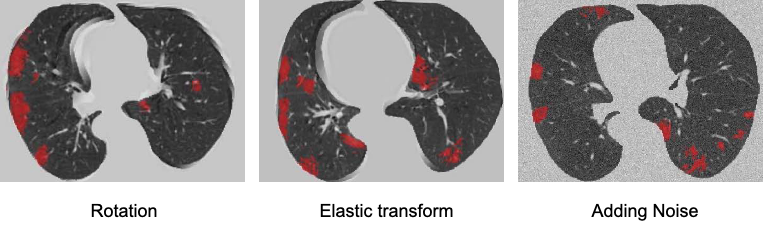
\includegraphics[width=\textwidth]{img/augment/rot_el_noise}
%	\caption{Augmenting the data}
%\end{figure}
%

%%%%%%%%%%%%%%%%%%%%%%%%%%%%%%%%%%%%
\chapter{Deep learning architecture}

\section{Network Architecture and Methodology}
Recall that in our project, due to large variation in the axial axis, we specified our problem into 2D segmentation task.\\

\subsection{Unet}
%TODO describe Unet here
We implemented a 2D Unet model as the baseline model, the original Unet structure is described in \ref{tab:OriginalUnet}. We further added a Batch Normalization layer before each activation better to alleviate covariance shift. The input image channel is one in our case because CT volumes are grey scale images.\\
We selected the input as original size because we want to reserve as much detail as possible. 
The input dimension is then (batch-size $\times$ 1 $\times$ 512 $\times$ 512), and the output dimension after softmax is (batch-size $\times$ 2 $\times$ 512 $\times$ 512) for the binary segmentation task, and we take an argmax to get the binary image the same size as the input.\\

\begin{table}
\centering
	\begin{tabular}{l c c c}
	\hline
	\hline
	Layer	&	input	&	output	&	channel	\\
	\hline
	Conv 3x3 + RELU	&	572	&	570	&	64	\\
	Conv 3x3 + RELU	&	570	&	568	&	64	\\
	Max Pool 2 $\times$ 2	&	568	&	284	&	64	\\
	Conv 3x3 + RELU	&	284	&	282	&	128	\\
	Conv 3x3 + RELU	&	282	&	280	&	128	\\
	Max Pool 2 $\times$ 2	&	280	&	140	&	128	\\
	Conv 3x3 + RELU	&	140	&	138	&	256	\\
	Conv 3x3 + RELU	&	138	&	136	&	256	\\
	Max Pool 2 $\times$ 2	&	136	&	68	&	256	\\
	Conv 3x3 + RELU	&	68	&	66	&	512	\\
	Conv 3x3 + RELU	&	66	&	64	&	512	\\
	Max Pool 2 $\times$ 2	&	64	&	32	&	512	\\
	Conv 3x3 + RELU	&	32	&	30	&	1024	\\
	Conv 3x3 + RELU	&	30	&	28	&	1024	\\
	up-conv 2 $\times$ 2	&	28	&	56	&	512	\\
	convs 1x1	&	56	&	54	&	512	\\
	convs 1x1	&	54	&	52	&	512	\\
	up-conv 2 $\times$ 2	&	52	&	104	&	256	\\
	convs 1x1	&	104	&	102	&	256	\\
	convs 1x1	&	102	&	100	&	256	\\
	up-conv 2 $\times$ 2	&	100	&	200	&	128	\\
	convs 1x1	&	200	&	198	&	128	\\
	convs 1x1	&	198	&	196	&	128	\\
	up-conv 2 $\times$ 2	&	196	&	392	&	64	\\
	convs 1x1	&	392	&	390	&	64	\\
	convs 1x1	&	388	&	388	&	2	\\
	\hline
	\hline
	\end{tabular}
	\caption{The Original Unet Architechture}
	\label{tab:OriginalUnet}
\end{table}

\subsection{Attention Gated Unet}
%TODO Describe Attention gate here
We used the original Attention Gated Unet architecture recommended in the paper \cite{??} that we added the Gate block before the skip connection concatenate to the upconvolution result in the corresponding layer.
An illustration is shown in figure \ref{fig:attention_gate}.
\begin{figure}
	\centering
	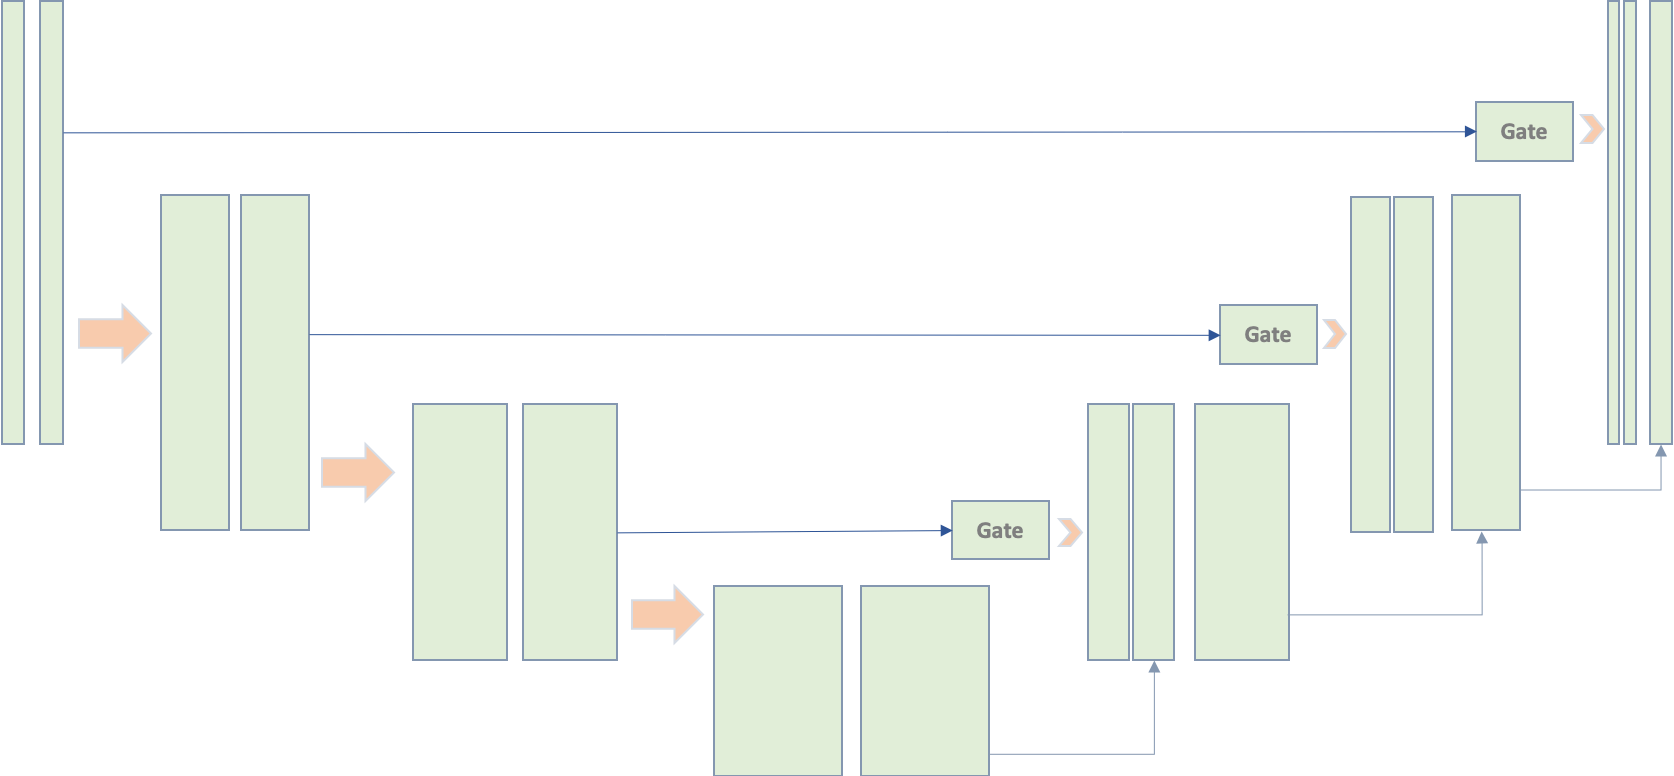
\includegraphics[width=0.8\textwidth]{img/Net_arch/attention_gate}
	\caption{An illustration of the attention block added in the Unet}	
	\label{fig:attention_gate}
\end{figure}

\subsection{Loss function}
\subsubsection{training objectives}
In this project, we used a combination of Foreground Soft Dice loss and Cross Entropy Loss. The justification of these combination is:
\begin{itemize}
	\item We consider CE loss converge fast for the background to learn the rough location of the segmentation
	\item We consider Foreground Dice only because for our highly imbalanced segmentation problem, adding background will vanish the loss and our segmentation target will not learn well.
\end{itemize}
Mathematically, we write our objective function as:
$$Loss=\frac{1}{I} \sum_{i=1}^{I} 1-\frac{2 \sum_{l=1}^{L} \sum_{c=1}^{C} p_{l}^{c} r_{l}^{c}}{2 \sum_{l=1}^{L} \sum_{c=1}^{C} p_{l}^{c}+r_{l}^{c}} - -\frac{1}{N} \sum_{c=1}^{N} \frac{1}{w_{c}} \sum_{l=1}^{L} r_{l}^{c} \log \left(p_{l}^{c}\right)$$

\subsubsection{Validation and testing scenario}
For Validating or testing the network, we used the foreground hard Dice Loss calculating the range of overlap.
$$Dice Loss = \frac{2|A \cap B|}{|A|+|B|}$$

\subsection{Transfer Learning}
As we discussed in the background chapter, the pretrained network from a source domain can serve as a good starting point for the issue especially when training data is not that sufficient. We make use of two different initializations one trained on our own and another one downloaded online, and fine tune the model on both the plain Unet and Attention Unet.
\begin{figure}
	\centering
	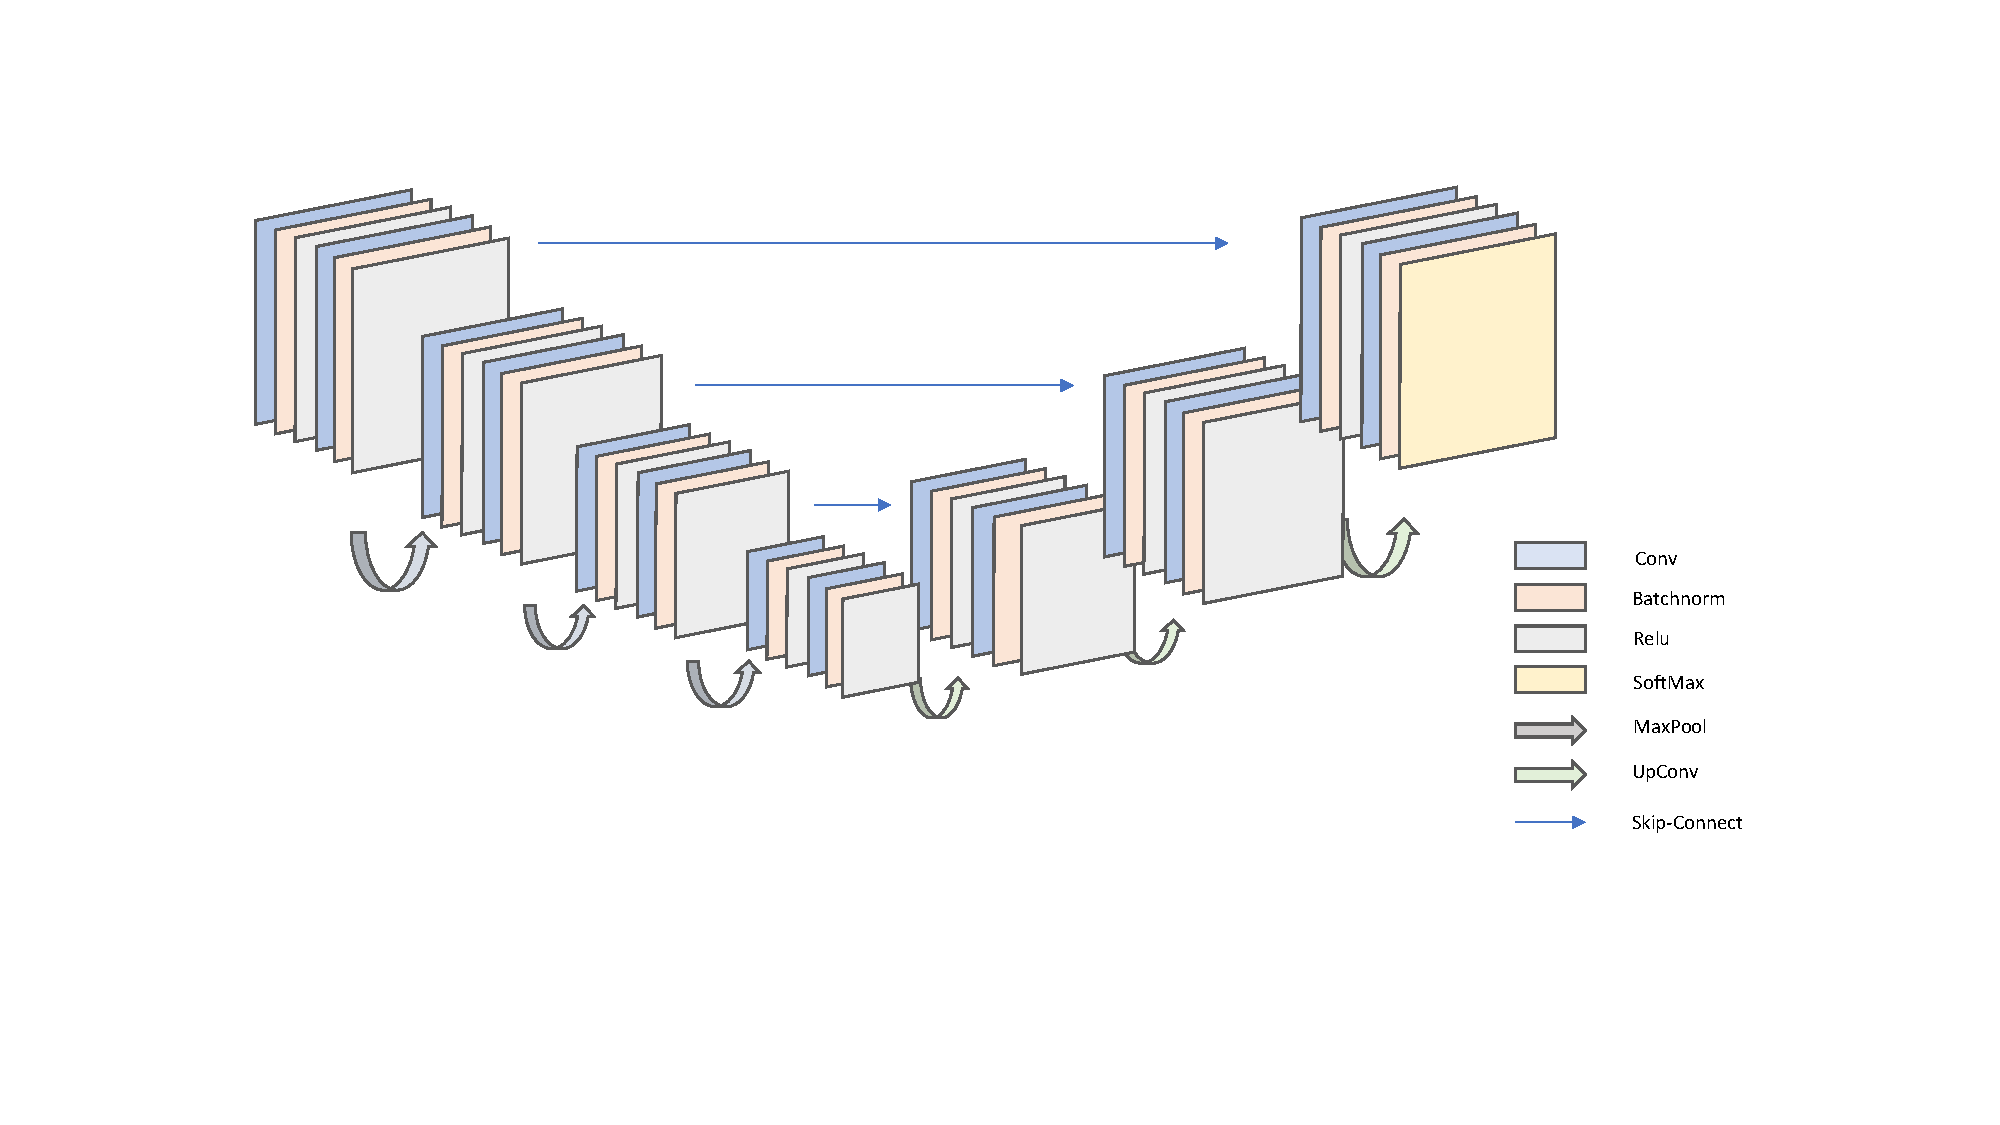
\includegraphics[width=0.8\textwidth]{img/Networks/Unet-train.pdf}
	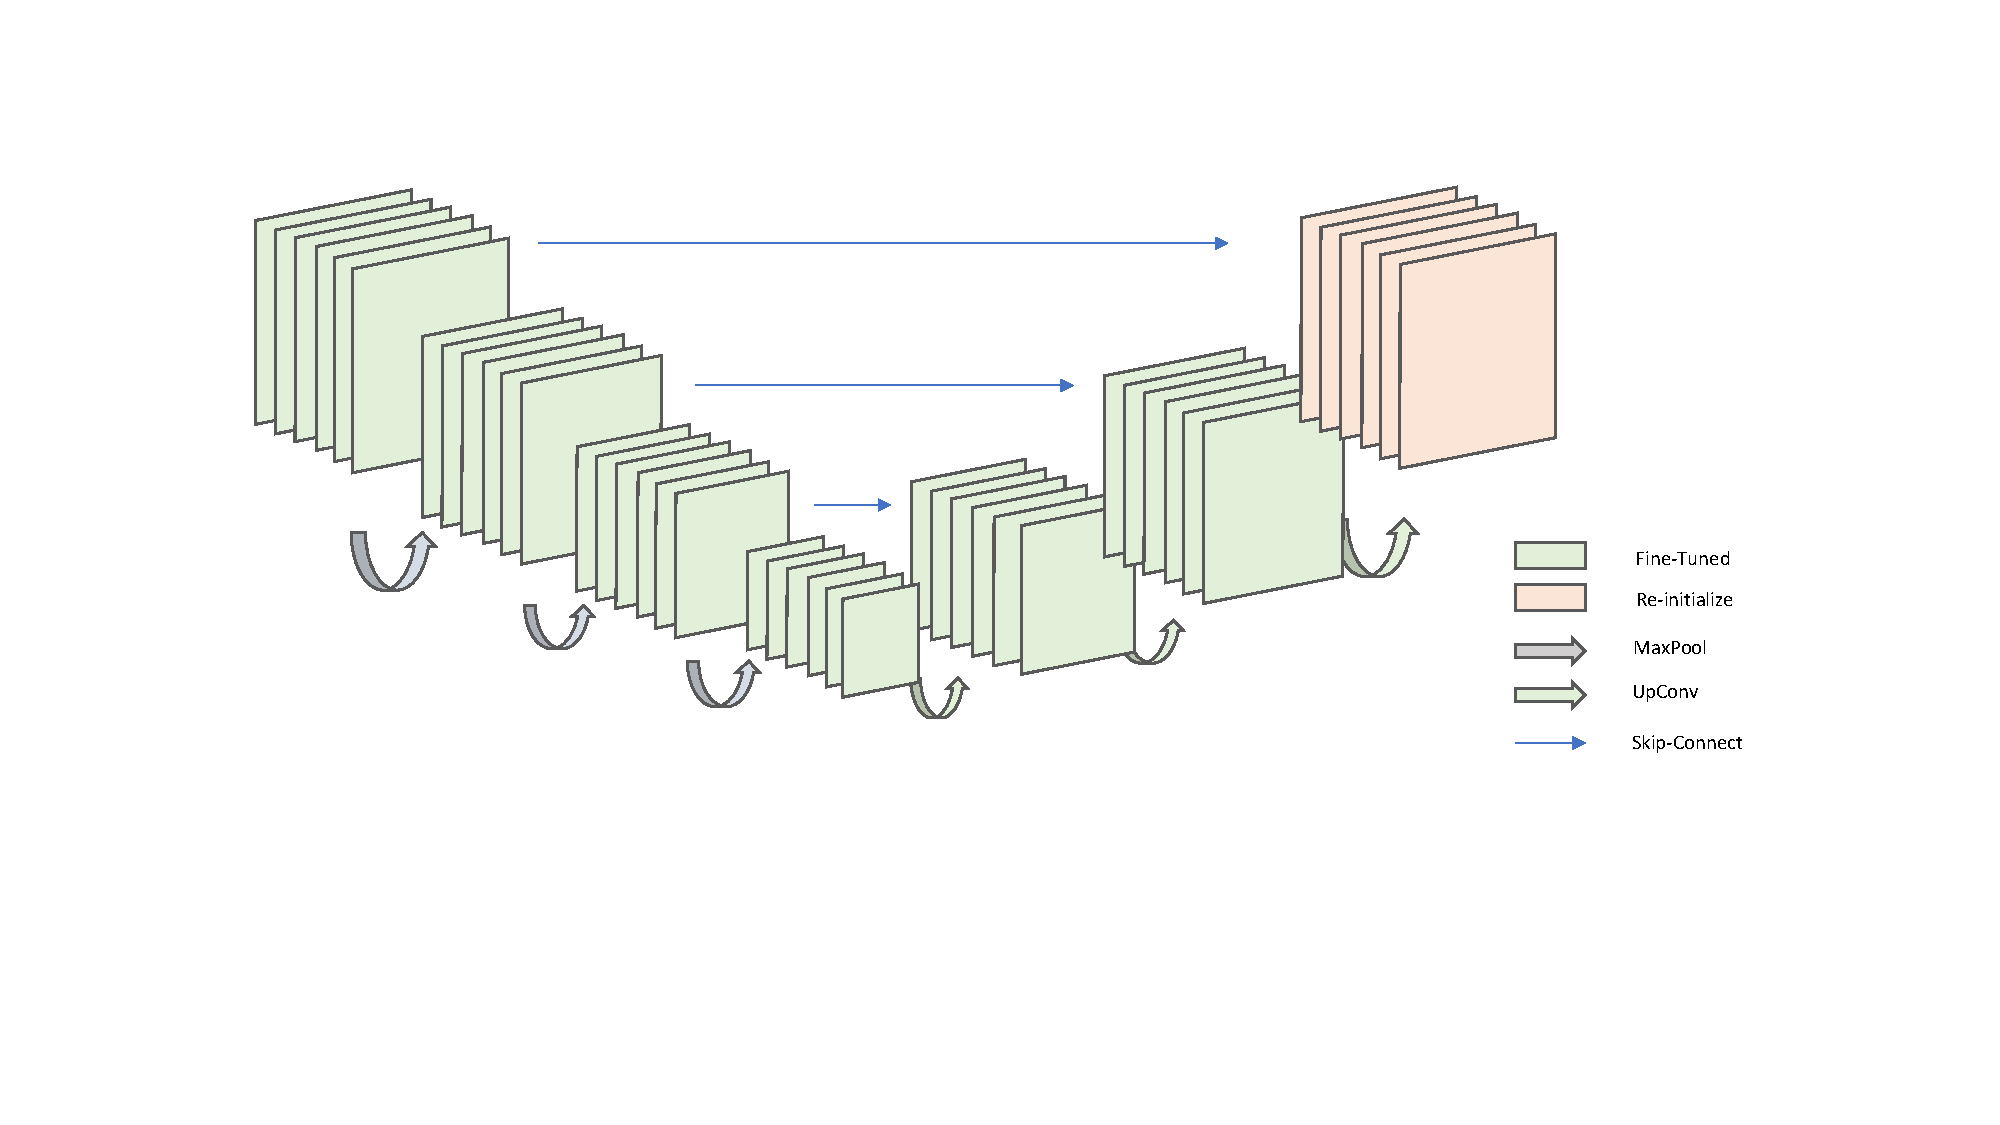
\includegraphics[width=0.8\textwidth]{img/Networks/Transfer-Finetune-all.pdf}
	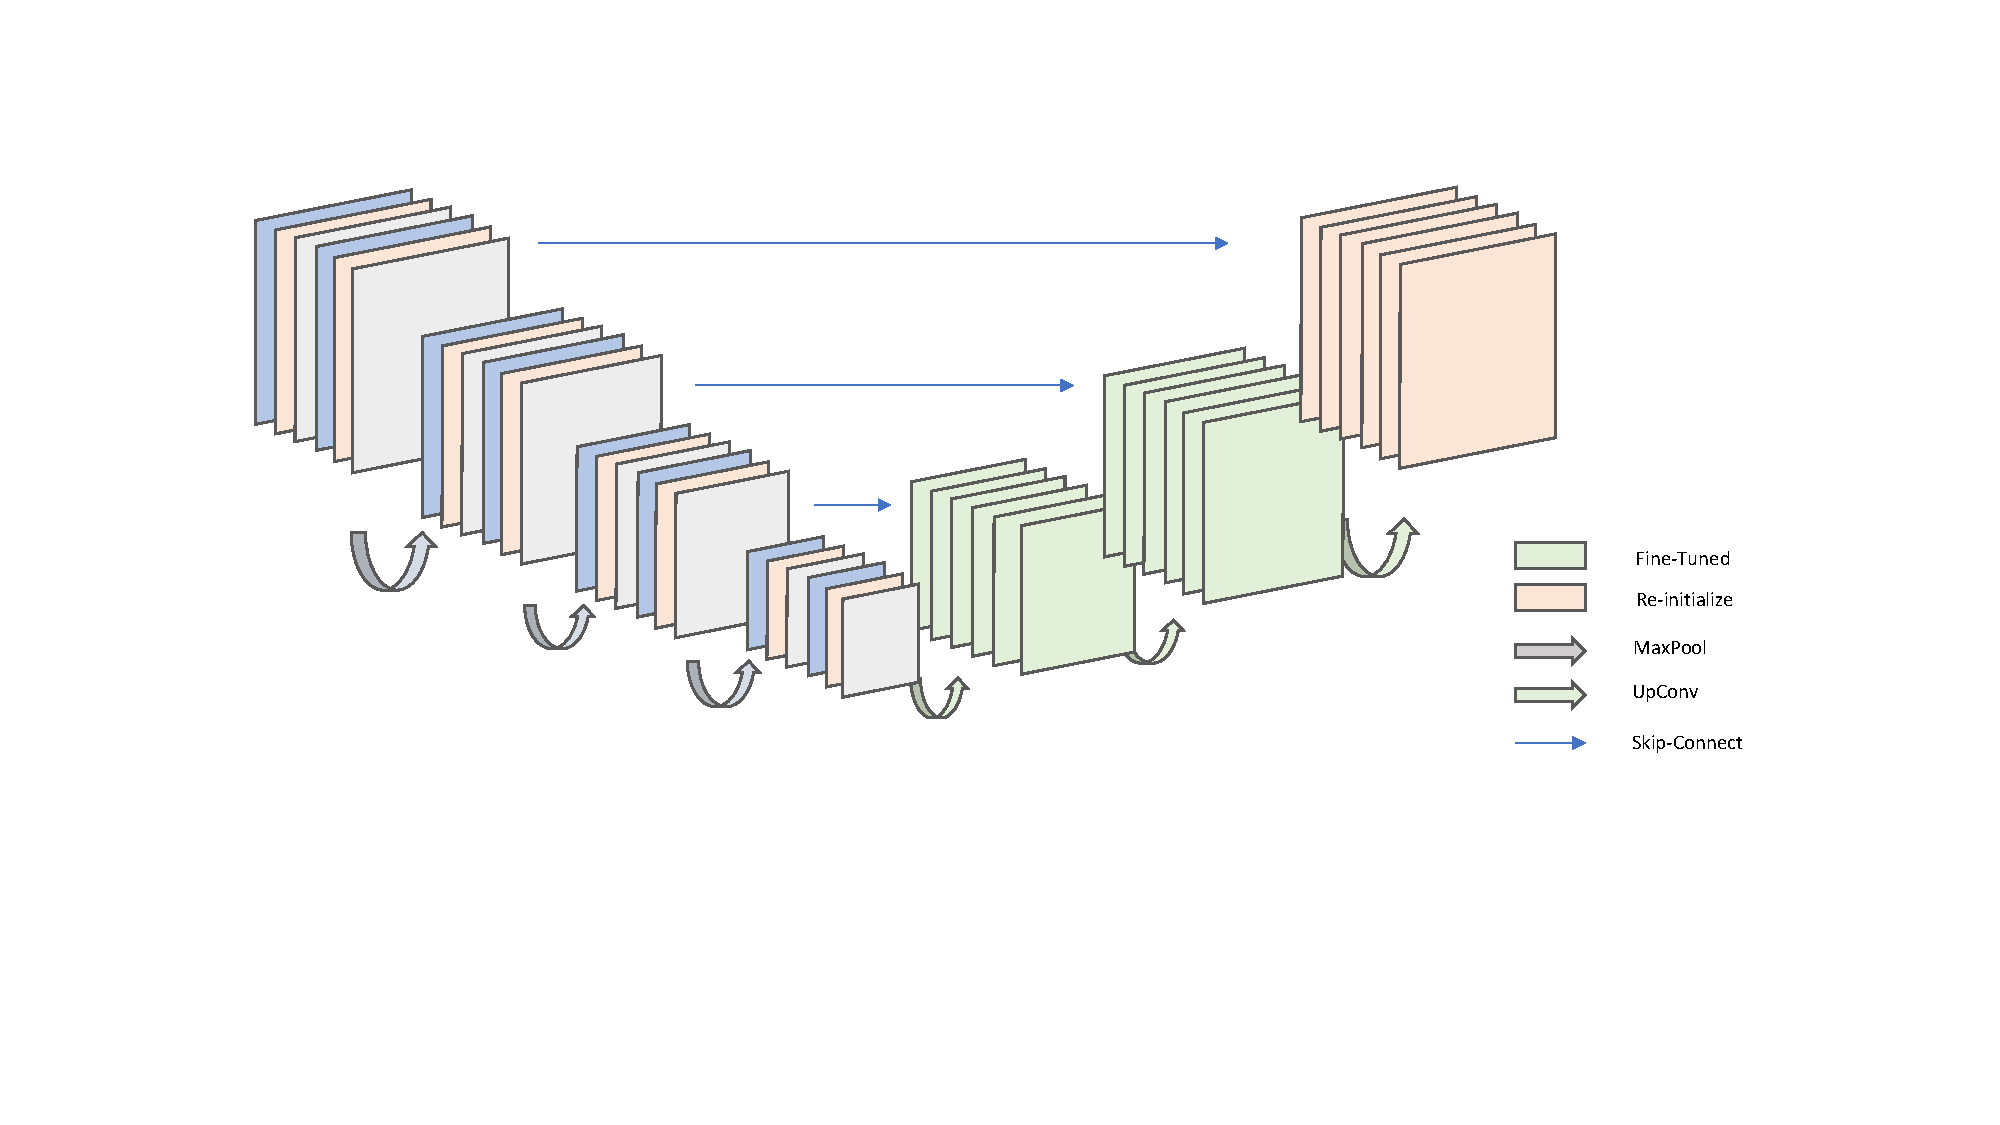
\includegraphics[width=0.8\textwidth]{img/Networks/Transfer-freeze-encoder.pdf}
	\caption{An illustration of Network structure used for pretraining and transfer-learning}
	\label{fig:transfer-learning-graph}
\end{figure}

\subsubsection{Pretraining}
For pretraining, we leverage two model initializations. We pretrained the model with the mixed Non-Covid lung Dataset, and we also used the weight initialization of the Model Genesis Dataset.
\begin{itemize}
	\item First the we pretrained the segmentation model using non-Covid dataset based on the assumption that the weights serves as good starting point for the fine-tuning stage.
	\item \color{red}Paper \cite{zhou_models_2019} pre-trained a 3D Unet-like model using several public dataset in the way that trained the model to restore image using destroyed image. The model was published in 3D \footnote{https://github.com/MrGiovanni/ModelsGenesis/tree/master/pytorch}. Since we did out experiment in 2D, we first load the 3D model and extract the layer weight. Then we flatten the weights into 2D as the initialization.
\end{itemize}

\subsubsection{Fine-Tuning}
We fine tuned the two pre-trained model using both of the initialization to train the Unet and the Attention Gate Unet architecture. We did experiment that allow the network to fine tune all or we freeze the encoder part. The justification of freezing the encoder can be further explained in the experiment section that SVCCA showed that the encoder showed less movement during fine-tuning.

\begin{enumerate}
	\item Freeze encoder: We freeze the first half of the encoder, and fine tuned the decoder except that we re-initialized the output layer.
	\item Fine-Tune-All: The whole network is fine tuned and the last block of convolutional layers was reinitialized.
\end{enumerate}

\begin{itemize}
	\item Fine-Tuning Unet: We directly load the trained model from the image and train the network and did the experiment with the two Fine-Tuning methods mentioned above.
	\item Fine-tuning Attention Gate: We consider that the attention gate for different domain are different, so for both of the fine-tuning methods, we take the encoder part only and append new decoder and attention gate to train from scratch.
\end{itemize}


\section{SVCCA implementation}

\section{presenting with unlabelled data}
Given that a larger amount of unlabelled data was published later in our project, we further investigated the semi-supervise segmentation area leveraging unlabelled dataset. We constructed a semi-supervise learning framework including psuedo labeling, and mean-teacher training with our loss function.
\subsection{Psuedo labeling}
We developed a new psuedo labeling framework that assign a reasonable label to the unlabelled samples.\\

We sampled both the labelled samples and the unlabelled images. For the labeled samples, we first get the bounding box of the segmentation mask, then enlarge the mask by a maximum of 10 pixels each side, and we sampled images within that bounding box.
For unlabeled images, we use the coarse 3D segmentation to generate the bounding box, and the bounding box was enlarged maximum of 15 pixels, we sample patches within the coarse bounding box.
To assign a noisy psuedo label to the cropped images, we take the encoder part of the trained 2D segmentation model and append a Global Average Pooling function. We then encode a dictionary of the annotated samples in the feature space.\\
\begin{figure}
	\centering
	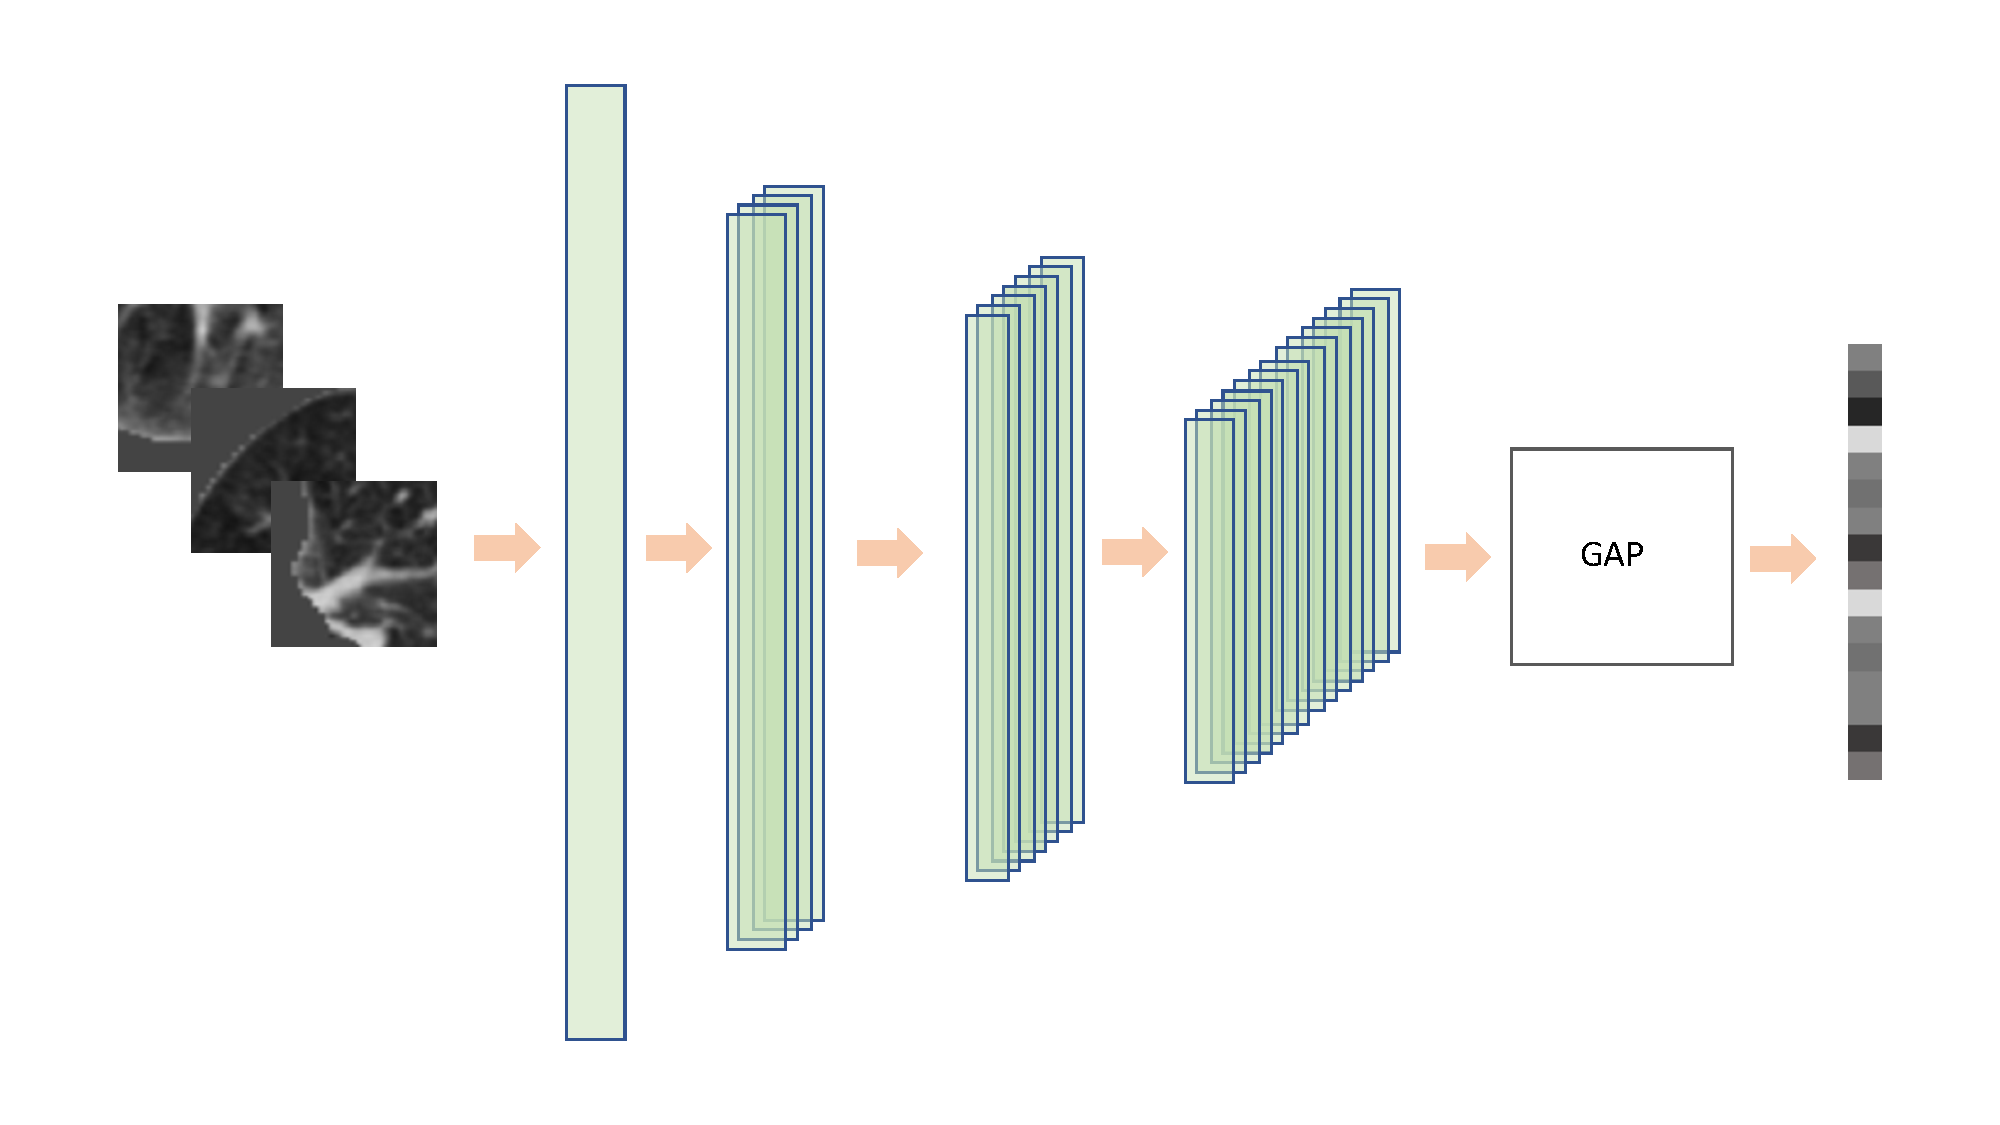
\includegraphics[width=0.9\textwidth]{img/semi-experiment/latent-space}
	\caption{An illustration of feature encoding process}
\end{figure}

For assigning noisy psuedo labels, given an unlabeled sample $I_{unlabeled}$ and its latent representation $Latent(I_{unlabelled})$, we calculated the pairwise cosine similarity and return the maximum cosine similarity score as the weight for this sample. 
$$\operatorname{similarity}(A, B)=\frac{A \cdot B}{\|A\| \times\|B\|}=\frac{\sum_{i=1}^{n} A_{i} \times B_{i}}{\sqrt{\sum_{i=1}^{n} A_{i}^{2}} \times \sqrt{\sum_{i=1}^{n} B_{i}^{2}}}$$
An illustration of the label assigning process is shown in figure \ref{fig:semi-label-assign}\\

\begin{figure}
	\centering
	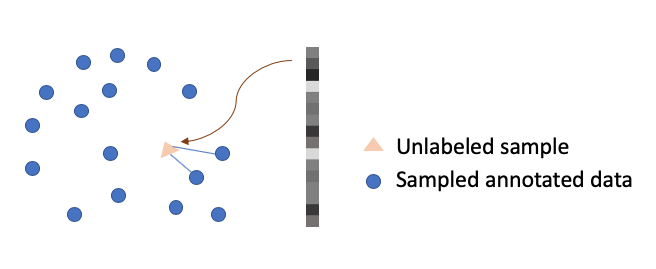
\includegraphics[width=0.8\textwidth]{img/semi-experiment/semi-label-assign}
	\caption{An illustration of label assigning to unlabelled samples}
	\label{fig:semi-label-assign}
\end{figure}

\subsection{Semi-supervise architecture}
After assigning reasonable psuedo labels to the samples, as we described in Chapter 2, we designed a Mean-teacher style model for the semi-supervise task.\\

The teacher model is the 2D Unet we described in section 4.1 transfered usining the non-covid dataset because we found that transfer learning give a better result as a intialization (detail in chapter 5), except that we only update the weight for no more than 10 epochs becuase we want the teacher model to be a bit more noisy than the converged model.\\

We first copied the trained weights to get the student model. For updating weights, we let the same patch go through the teacher and student model, and calculate the prediction consistency, we calculate a degraded dice score on the student network prediction with the pseudo label, and we set the weight to 1 * Dice Loss for a lighter penalization. The weight decreased every 5 epochs by 0.8. The student network weights are updated per batch (or observation) and the teacher model is update once per epoch.                         

 Figure \ref{fig:mean-teacher-training} showed an illustration of the weight update process using this framework.
 %TODO insert here the formal loss function
\begin{figure}[h]
	\centering
	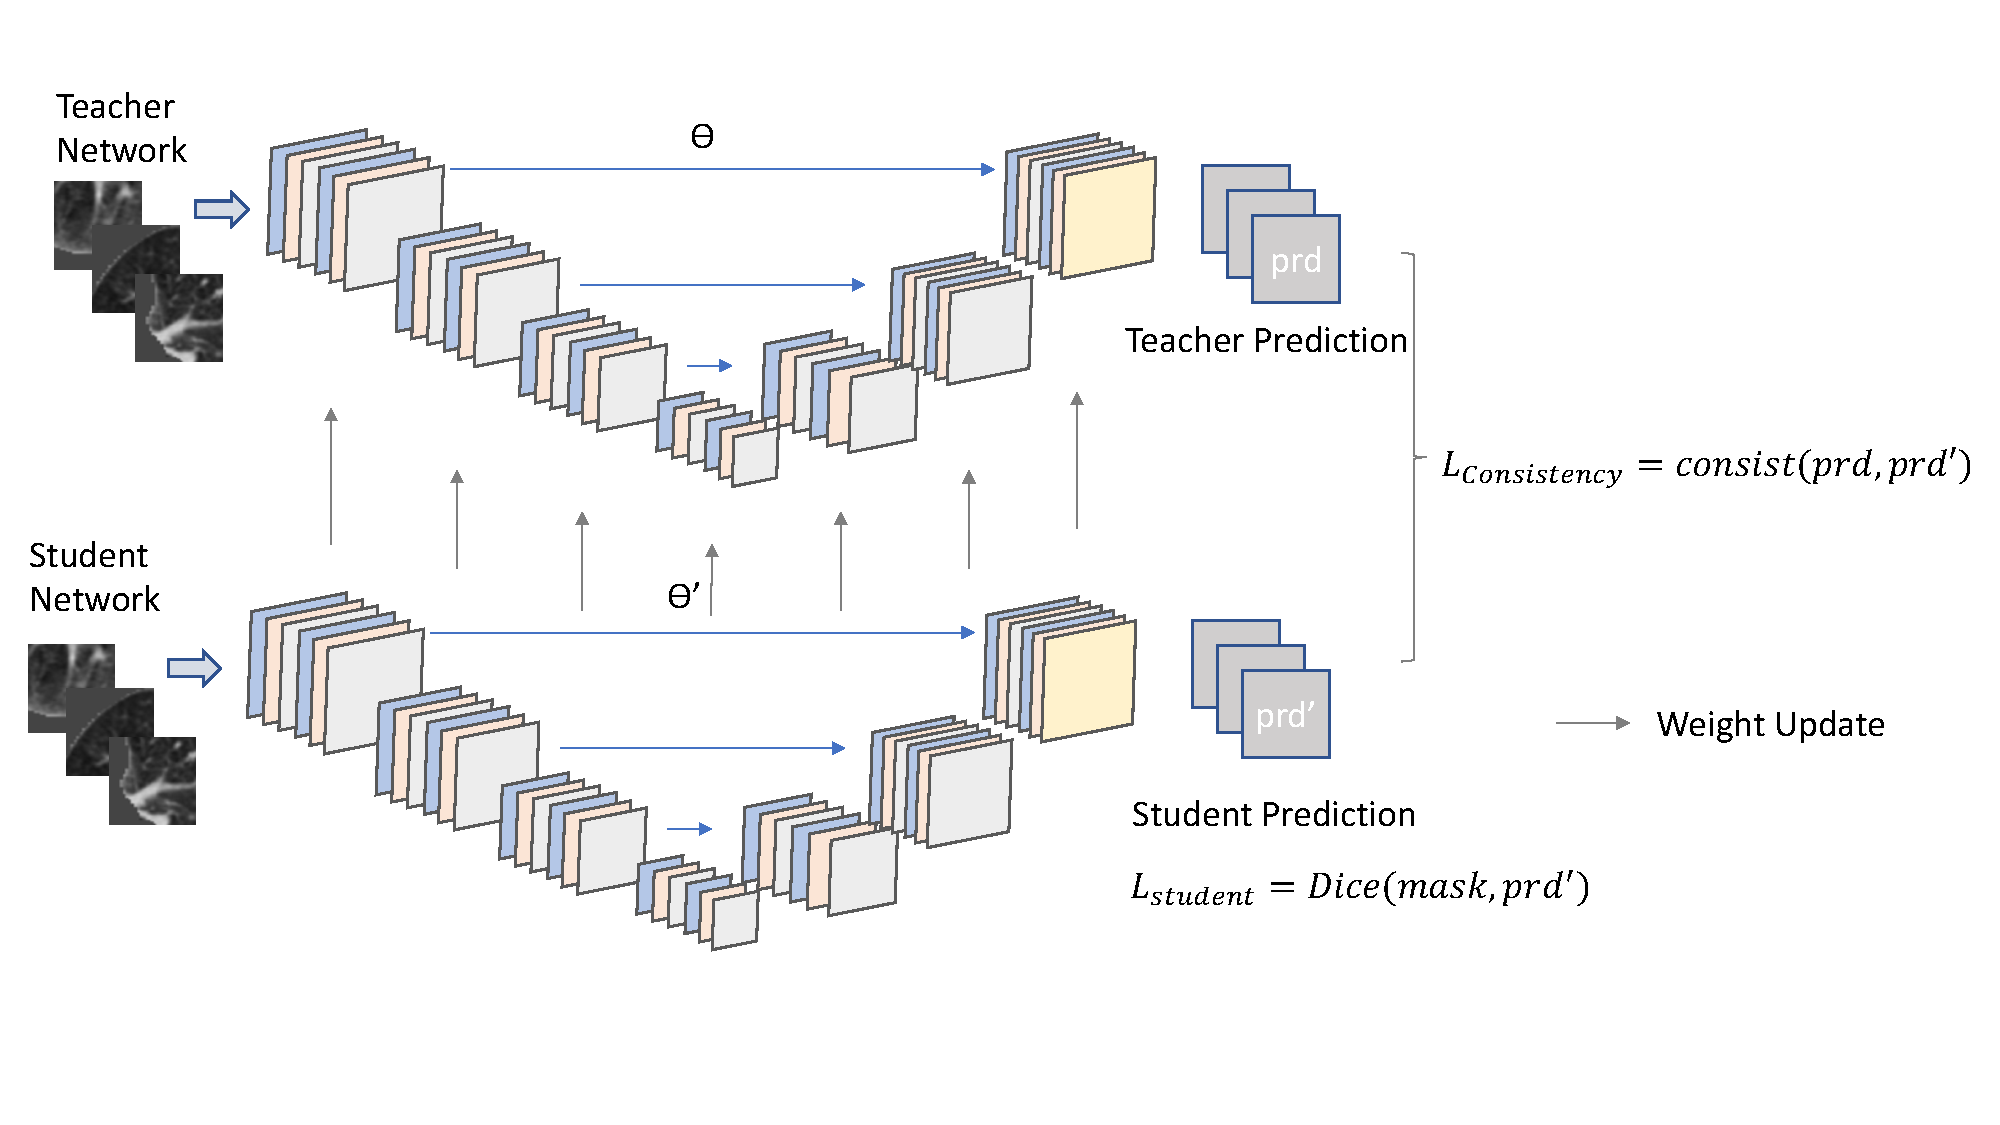
\includegraphics[width=\textwidth]{img/Networks/mean-teacher-net}
	\caption{The design of network model for our semi-supervise setup}
	\label{fig:mean-teacher-training}
\end{figure}

\subsection{Loss function for training}
Mathemartically, we write the Loss function as

$$L_{train} = L_{consistency} + L_{segmenation}$$
$$L_{train} = CE(prd_{teacher}, prd_{student}) + Dice(prd_{student}, mask) $$
\subsection{Validation and testing}
For the evaluation, we used the Dice Loss as we did in section 4.1.


%%%%%%%%%%%%%%%%%%%%%%%%%%%%%%%%%%%%
\chapter{Experiment}

\section{Experiment}
A good model, especially facing with small sample segmentation, should generalize well instead of overfitting on a small number of training data. The whole point of data augmentation, adding noise, etc, is to improve the generalizability of the trained neural network so that for the unseen data, the model predict reasonably well.\\

Due to the limited ability of the GPU resource available, tuning hyper-parameters using grid search is too inefficient. Thus in our experiment, we leveraged the optimizer scheduler in PyTorch so that starting from the learning rate starts from $lr=2\times10^{-4}$ and decreased to 0.8 * lr every 25 epochs so that the learning rate approach 0 in the later training stage.  
\begin{enumerate}
	\item \textbf{learning rate}
	\item \textbf{Optimizer:} We used Adam optimizer considering that Model Genesis, winning solution for NSCLC segmentation as well as other well known solutions used the model optimizer.
	\item \textbf{Epochs:} The maximum number of epochs for training is 500. However, each epoch we validate the result and the best model was saved throughout the training process. We count the number of continued non-improving epochs, and when it reached 30 epochs, the training progress terminated automatically.
	\end{enumerate}

\section{With Fully labelled data}
We first consider training on a small dataset and all of them are labelled with segmentation masks, because this is the case during the first few months of this project when only 20 volumes of the Covid lungs from the Covid Segmentation benchmark were publicly available, later in July 2020, MosMed published a new dataset containing 50 labeled slices.

\subsection{Experiment Setup}
To fully leverage the Covid Dataset, we combined the 20 volumes in Covid Segmentation bechmark and the 50 volumes MosMed Dataset. We randomly selected 20 volumes for testing, and further split the 50 remaining volume into 5 fold for cross validation. Smaller sample: One fold (10 volumes) for training; Normal training: Four fold (40 Volumes) for training.
Note that since we cannot do anything to the various slice thickness, we sliced the volume into 2D.

\subsection{Best results}
For the segmentation of infection area using \textbf{fully labelled sample only}, we achieved Dice score (DSC) on the training set (50 volumes sliced in 2D) of 99.0321\%, 80.3601\% on the validation set and 79.9356\% on the testing set. All the volumes was preprocessed as described in Section 3 and augmented the data using random rotating, and elastic transformation and {\color{red}mix up augmentation} on the training set only.

\subsection{Training}
We compared the model trained from scratch and with transfer learning in this experiment. More specifically, we experimented two transfer learning intialization in this section. First we trained the Binary segmentation task with the images from NSCLC and MSD dataset, then the model was fine tuned using two different methods suggested in work \cite{wang_improving_2019}: Fine-Tuning all layers (reinitialize the last layer), and Fine-Tuning only the Decoder, shown in figure \ref{fig:transfer-learning-graph}.\\

%\begin{figure}
%	\centering
%	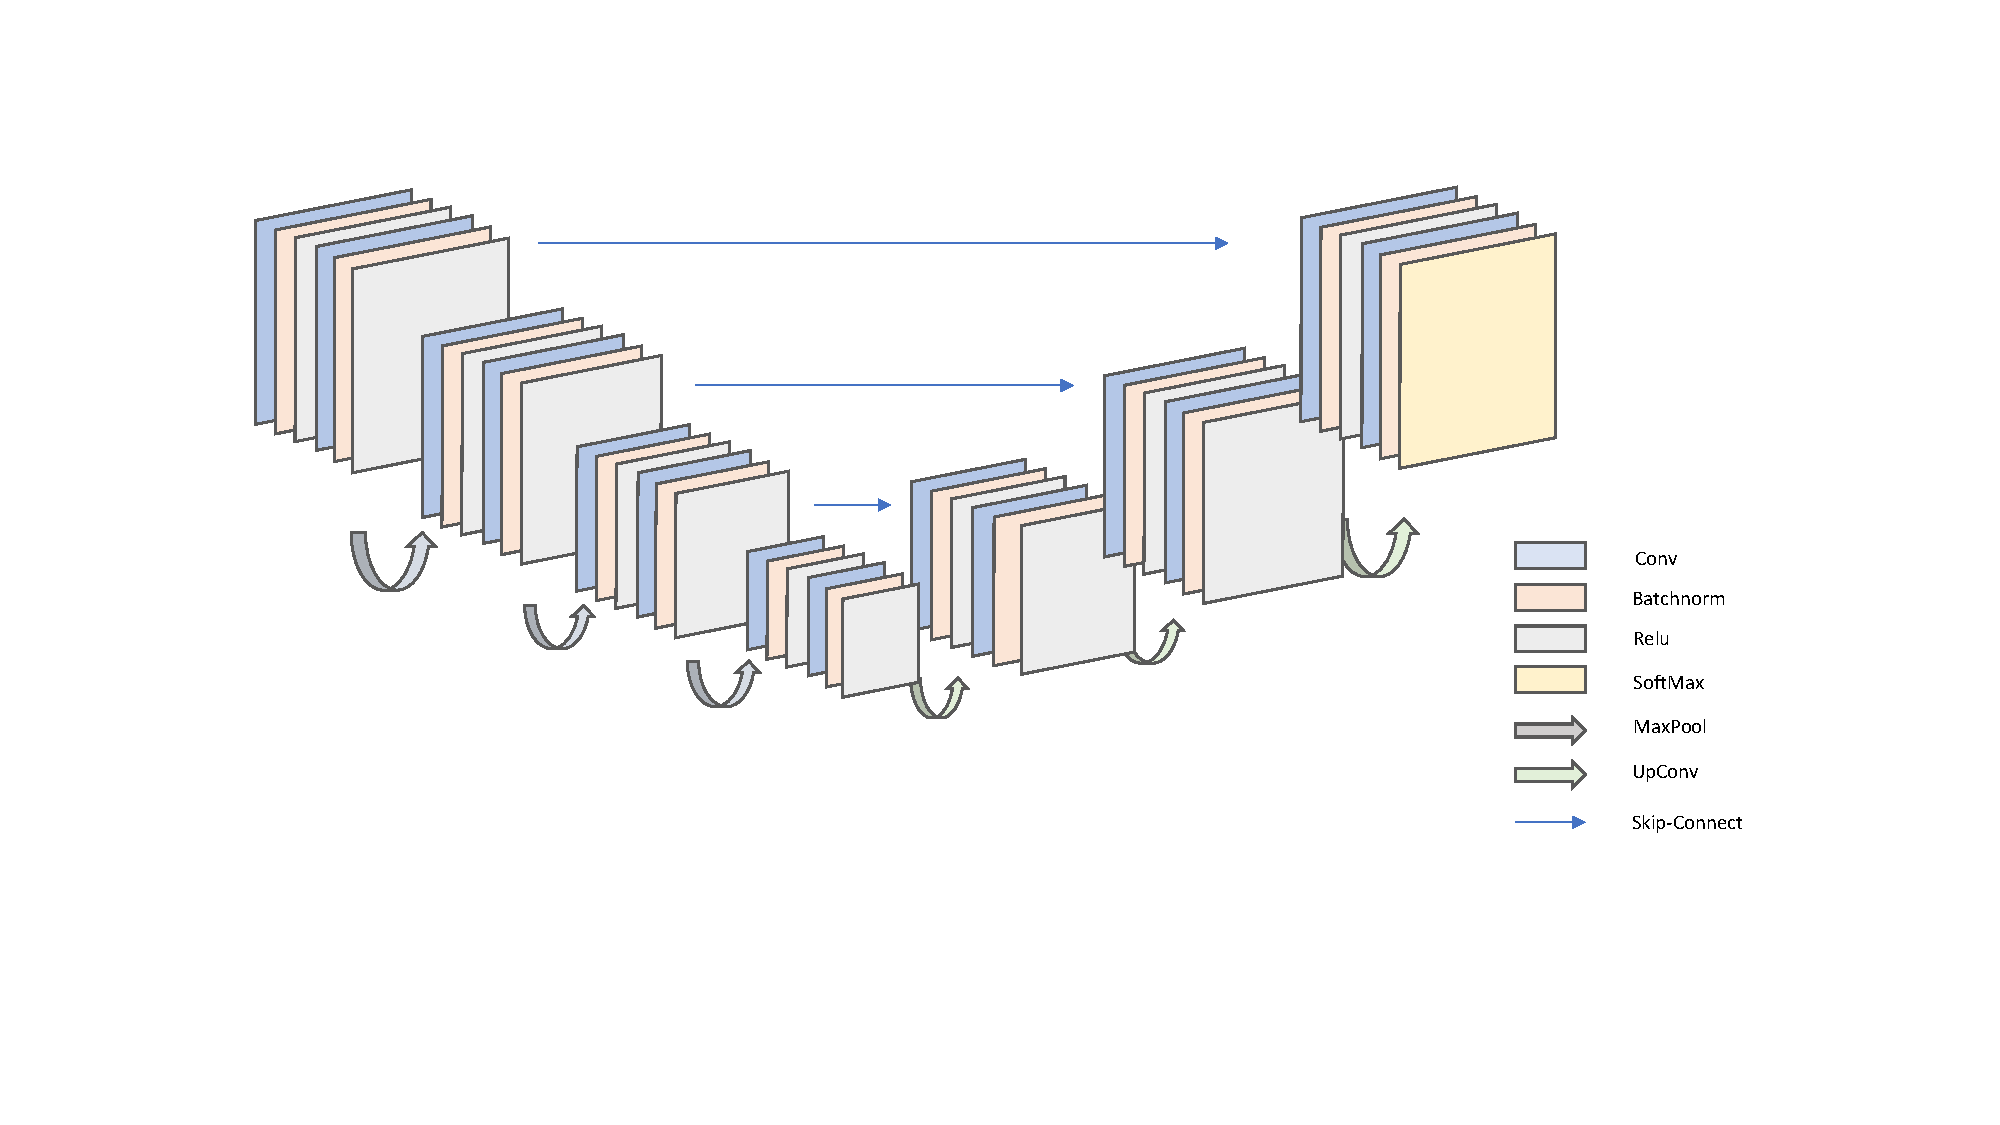
\includegraphics[width=0.8\textwidth]{img/Networks/Unet-train.pdf}
%	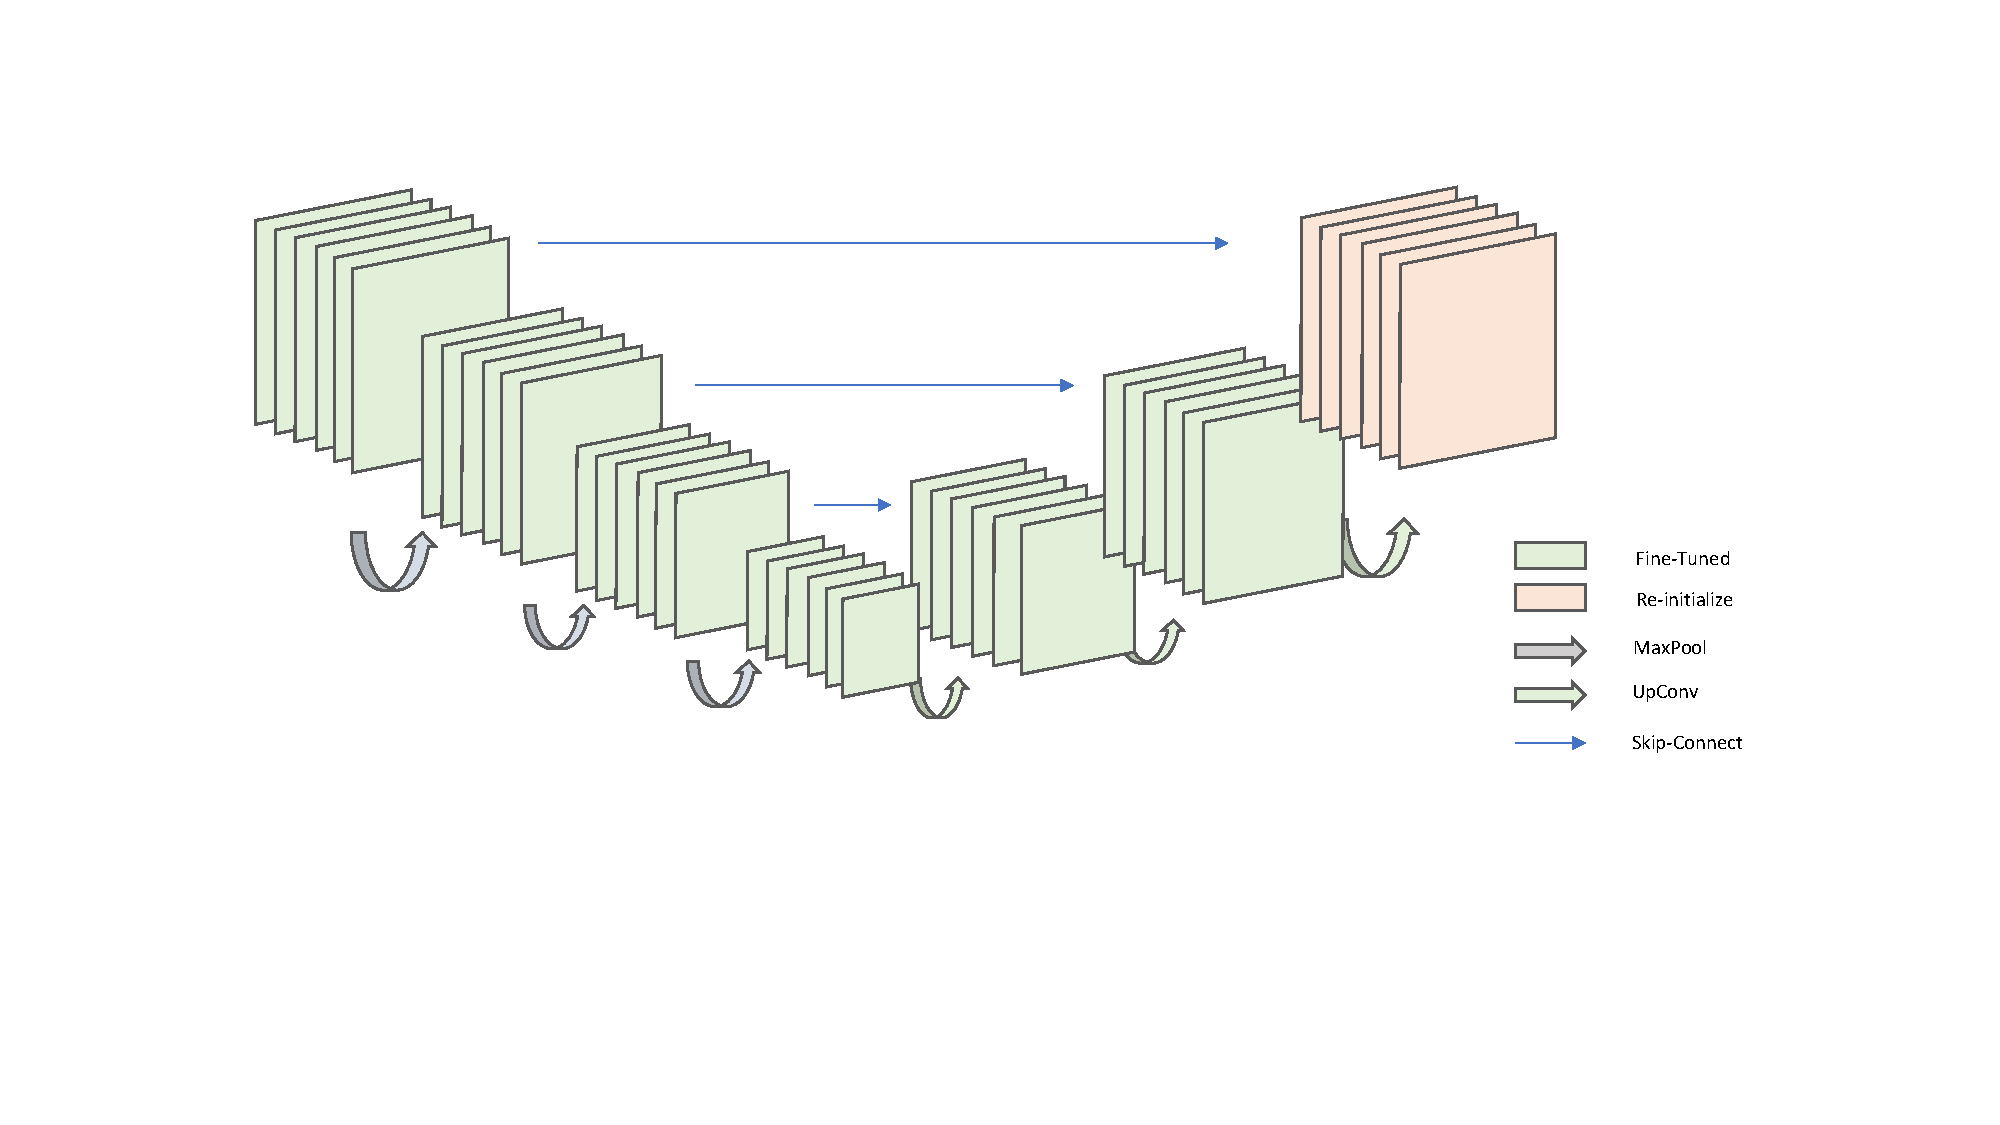
\includegraphics[width=0.8\textwidth]{img/Networks/Transfer-Finetune-all.pdf}
%	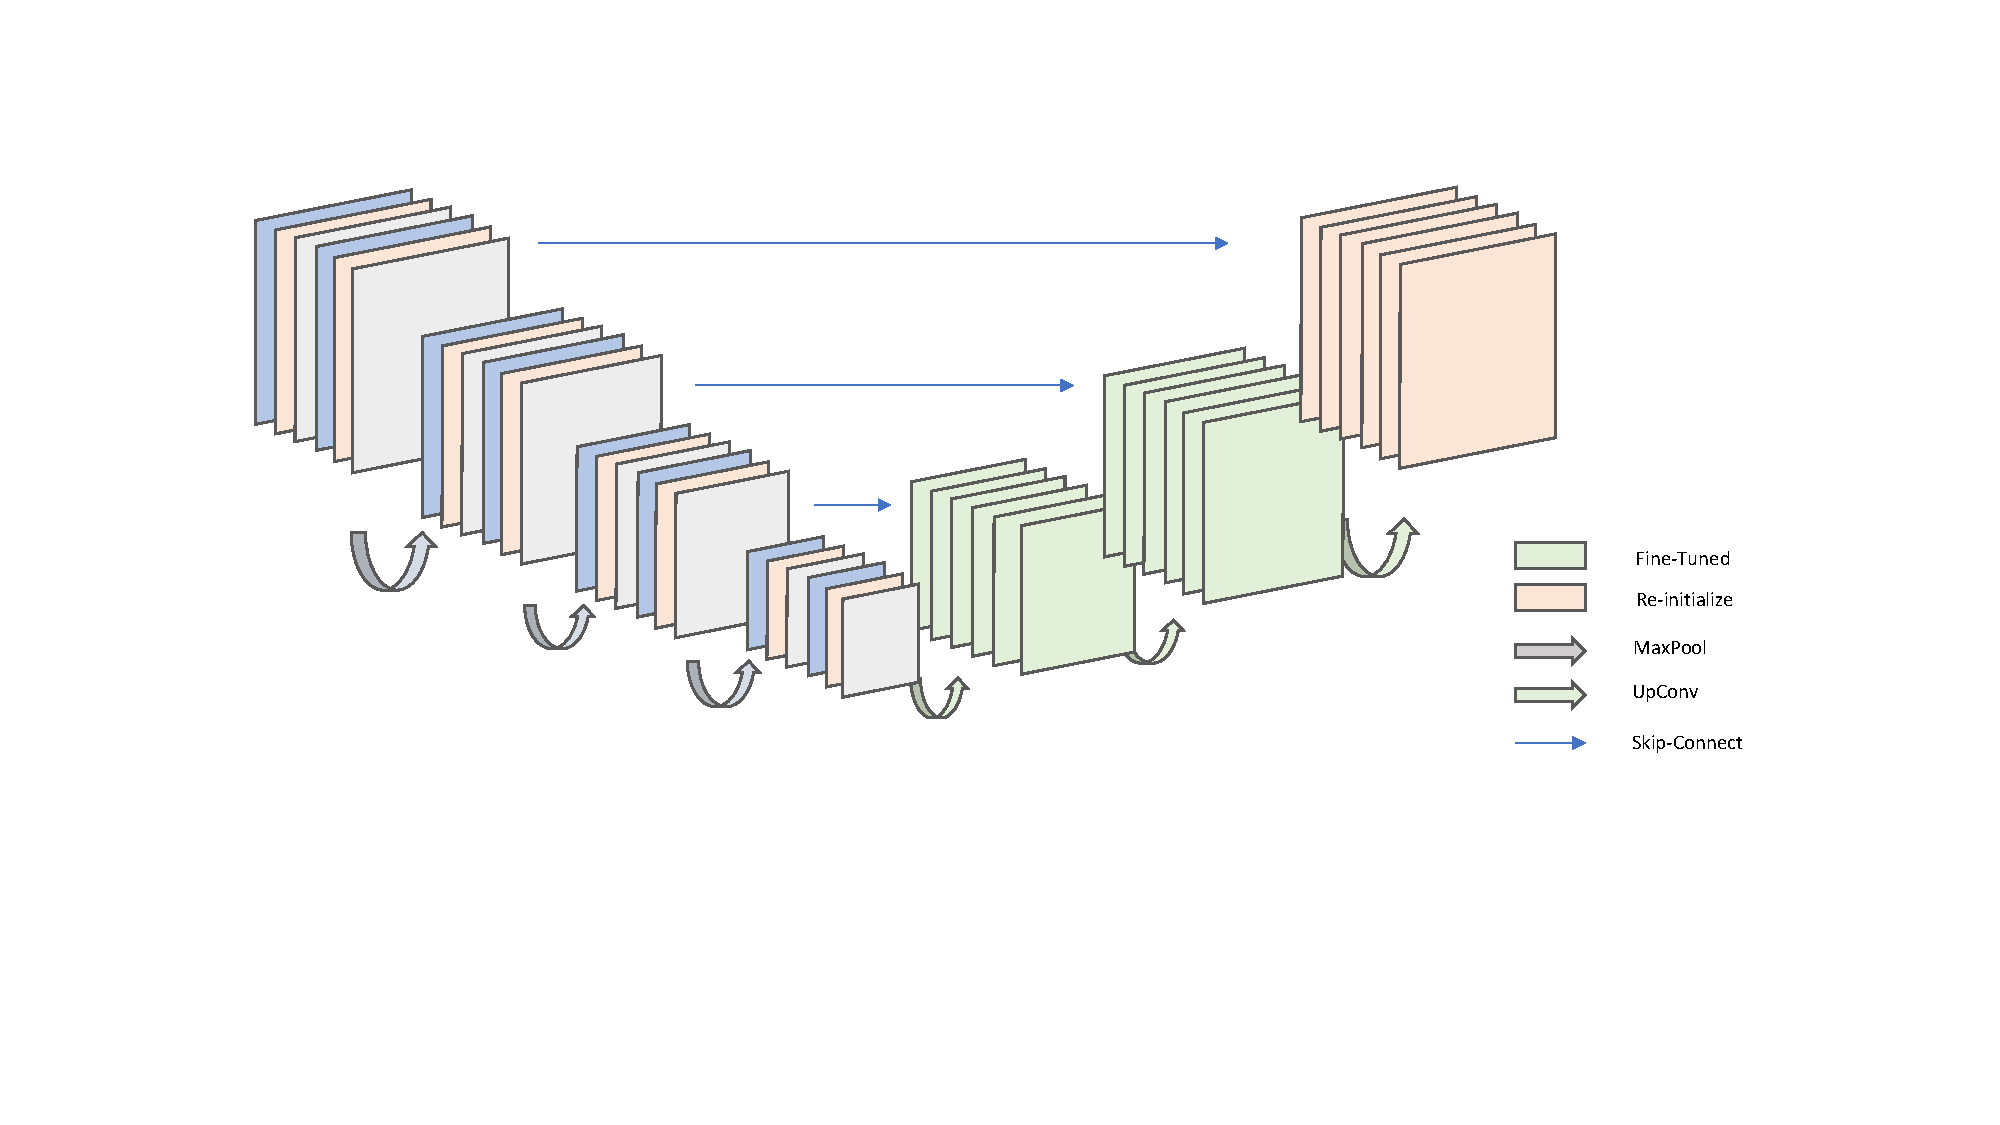
\includegraphics[width=0.8\textwidth]{img/Networks/Transfer-freeze-encoder.pdf}
%	\caption{An illustration of Network structure used for pretraining and transfer-learning}
%	\label{fig:transfer-learning-graph}
%\end{figure}
%
%\textbf{Pretraining with NSCLC and MSD Dataset}\\
%
%First the we pretrained the segmentation model using non-Covid dataset based on the assumption that the weights serves as good starting point for the fine-tuning stage. Figure \ref{fig:filtered_Lung} plots the validation loss every 10 epochs.\\
%%\begin{figure}
%%	\centering
%%	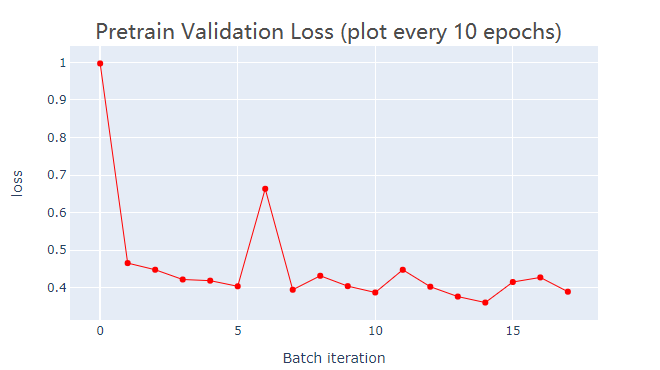
\includegraphics[width=0.8\textwidth]{img/Loss_curves/Pretrain_lungs_plot}
%%	\caption{Validation Loss with pre-training on non-Covid Lung dataset}
%%	\label{fig:pretrain_lungs}
%%\end{figure}
%
%\textbf{Fine Tuned with Model Genesis:}\\
%
%{\color{red}Paper \cite{zhou_models_2019} pretrained a 3D Unet-like model using several public dataset in the way that trained the model to restore image using destroyed image. The model was published in 3D \footnote{https://github.com/MrGiovanni/ModelsGenesis/tree/master/pytorch}. Since we did out experiment in 2D, we first load the 3D model and extract the layer weight. Then we flatten the weights into 2D as the initialization.}\\
%
%\textbf{Freezing encoder:}
%We freeze the first half of the encoder, and fine tuned the decoder except that we re-initialized the output layer.\\
%
%\textbf{Fine-Tune-All:}
%The whole network is fine tuned and the last block of convolutional layers was reinitialized. \\

\begin{table}[h]
	\centering
	\begin{tabular}{l  c c c c}
	\hline
	\hline
	Unet	&		&	Train	&	Validation	&	Test	\\
	\hline
	From Scratch	&	10-40 split	&	0.9894	&	0.7012	&	0.6893	\\
			&	40-10 split	&	0.9705	&	0.8119	&	0.8012	\\
	Fine Tune Decoder	&	10-40 split	&	0.9771	&	0.7963	&		\\
			&	40-10 split	&	0.9693	&	0	&		\\
	Fine Tune All	&	10-40 split	&	0.9802	&		&		\\
			&	40-10 split	&	0.9562	&		&		\\
	\hline
	\hline
	Attention gated Unet	&		&	Train	&	Validation	&	Test	\\
	\hline
	From Scratch	&	10-40 split	&	0.9904	&		&		\\
				&	40-10 split	&	0.9710	&		&		\\
	Fine Tune	&	10-40 split	&	0.9521	&		&		\\
				&	40-10 split	&	0.9512	&		&		\\
	Fine Tune All	&	10-40 split	&	0.9608	&		&		\\
				&	40-10 split	&	0.9611	&		&		\\	
	\hline
	\hline
	\end{tabular}
	\caption{Training with fully labeled Dataset}
	\label{tab:fully-label-result}
\end{table}
	


\subsection{SVCCA analysis on transfer learning}

\subsubsection{Network convergence during training}
We compared the convergence on each layer throughout the training process on the segmentation model. \cite{transfusion} reported that the network converged bottom up for a classification task during training. However, this is not exactly the case in our segmentation model.\\

\textbf{Network convergence with random initialization}\\

We first want to analyze the change of network layers from random initialization towards convergence using the SVCCA tool. We iterate through the dataloader and validate every 100 epochs and save the model if the result yield better performance.\\
\begin{figure}
	\centering
	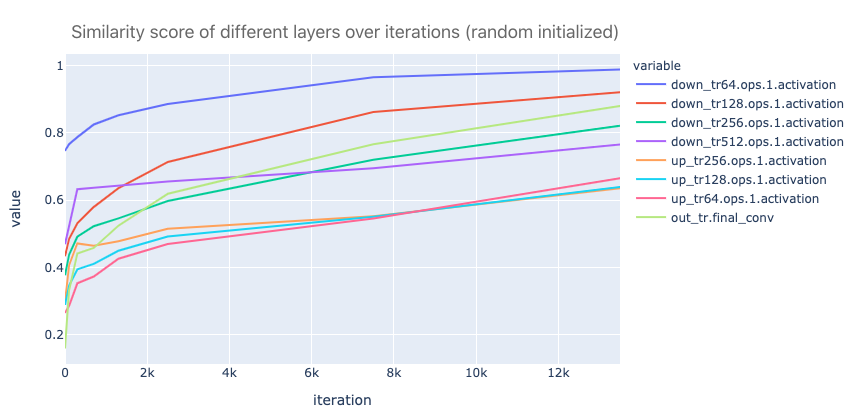
\includegraphics[width=0.8\textwidth]{img/SVCCA/CCA_score_scratch.png}
	\caption{CCA similarity score of each layer over training iterations (randomly initialized)}
	\label{fig:random_init_converge}
\end{figure}

Figure \ref{fig:random_init_converge} plots the similarity of latent space of each network layer using random initialization. 
\begin{itemize}
	\item We observed that, in general, encoder converged faster than decoder.
	\item Suprisingly, the first down convolution layer moved less comparing the initialization to the converged model.
	\item The similarity score in the output layer converged slightly faster than the other decoder part. Our explanation is that, the model performance (accuracy) increased faster in the first few number of iterations then slowly improved throughout the training.
	\item Although the similarity of the several Up-Convolution in the decoder part kept changing in the later stage of training, the output layer(out\_tr.finalconv in figure \ref{fig:random_init_converge}) did not moved much. One implication is that, Neural Network may learn different latent feature space while giving similar performance with respect to the accuracy.
\end{itemize}

\begin{figure}
	\centering
	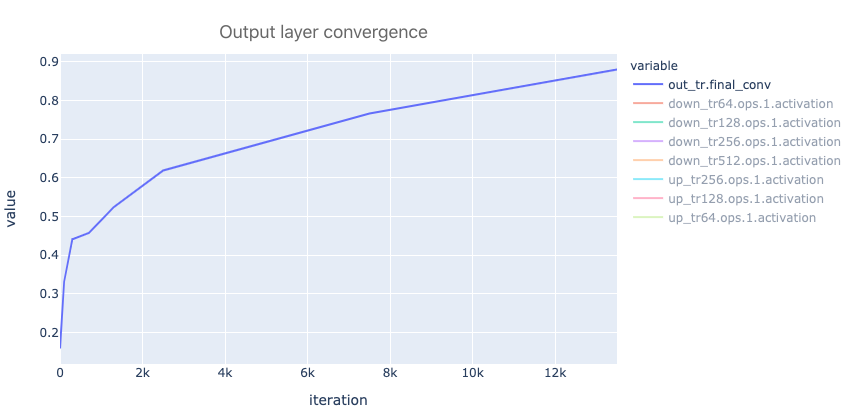
\includegraphics[width=0.8\textwidth]{img/SVCCA/from_scratch_output_layer.png}
	\caption{Filtering out the output layer convergence}
	\label{fig:random_init_converge}
\end{figure}

%\textbf{Train from scratch and transfer learning}\\
%We first compared the model before and after transfer learning. We saved the model that trained from scratch using the Covid dataset and the model pretrained using Lung dataset then fine-tuned to Covid dataset

\textbf{Network convergence during Fine-tuning}\\

The question we asked is: \textbf{Is the convergence similar to random initialization when we have a pre-trained model?}
To test the convergence, we repeated the experiment in the previous section: Starting from a pre-trained model, we iterate through the Dataloader (containing 40 volumes sliced into 2D from the Axis view) and validate every 100 iterations. We saved the model of that epoch if the validation accuracy reported a better performance. Figure \ref{fig:transfer-convergence} plots the CCA similarity score of each saved model compared with the converged model.

\begin{figure}
	\centering
	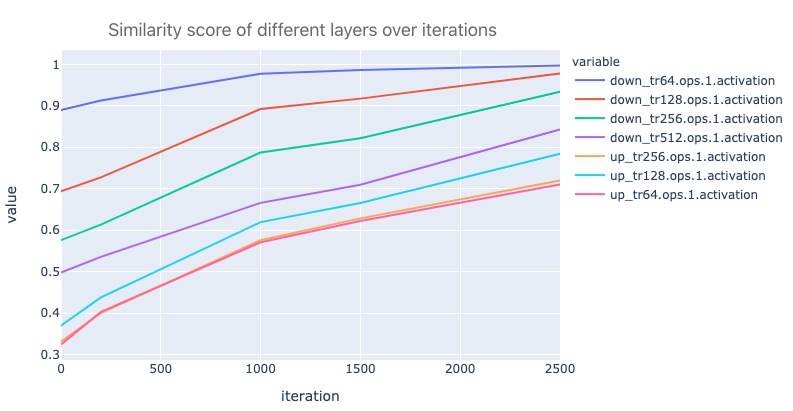
\includegraphics[width=0.8\textwidth]{img/SVCCA/CCA_score_transfer_learning}
	\caption{CCA similarity score of each layers over iterations during Fine-tuning}
	\label{fig:transfer-convergence}
\end{figure}

Comparing the similarity of feature map in the segmentation model, we observed the following behaviour:
\begin{itemize}
	\item In the Encoder part, lower layers converged faster compared to higher layers. Specifically, down covolution reported higher similarity score from the beginning compared with the similarity score obtained when we trained from scratch
	\item Layers in the Decoder observed convergence almost at the same time.
\end{itemize}

\subsubsection{Feature space comparison for transfer learning} 
%%TODO Change the title here
Another question we want to discuss is: \textbf{How much did the model move given the amount of data it observed during the Fine-Tuning?}\\

\textbf{A larger amounts of data:}\\
Figure \ref{fig:transfer-convergence} shows that, although all layers output seen a higher similarity score as the iteration number increase, 
Down-Convolution layers in the Encoder moved much less compared to the rest of the model, yielding a slightly better feature reuse during Fine-Tuning, and the feature reuse decreased from lower layers to higher layers. The Decoder, however, gives a much lower similarity score (lower than 0.5) comparing the pre-trained initialization to the converged model. Figure \ref{fig:layer-wise-comparison} compared the layer-wise feature space similarity which showed the similar obeservation.

\begin{figure}
	\centering
	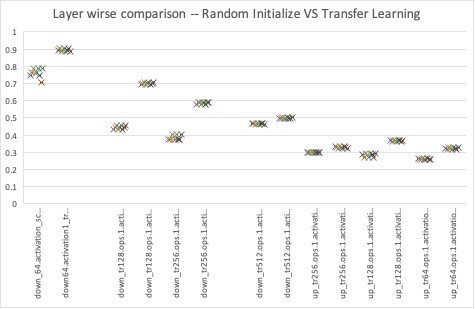
\includegraphics[width=0.8\textwidth]{img/SVCCA/randvstansfer-init2converge.png}
	\caption{Layer-wise Comparison during training}
	\label{fig:layer-wise-comparison}
\end{figure}

{\color{red}{We then trained the model using only 5 volumed sliced into 2D......}}

\section{With unlabeled data}
We then consider leveraged unlablled data because in mid July, MosMed published unlabelled CT volumes. Thus, we continued our experiment to leveraged the unlabeled dataset. 
 We first fine tune a pre-trained model on the annotated dataset, take the encoder of the network. We cropped patches from the unannotated images, assign noisy label to them and train a mean-teacher style network using those cropped patches

\subsection{Experiment Setup}
Apart from the labelled datset described in section 5.2, we downloaded 200 unlabeled volumes and first preprocessed the CT volumed as we described in chapter 3.

\subsection{Training a coarse 3D segmentation}
The purpose of leveraging unlabelled data during training is to improve the generalization of the network so that it generalize better on unseen data. We want to crop more infection area to guide the segmentation model, so we first train a coarse 3D segmentation to generate a 'rough mask' of the image to guide the segmentation.
% TODO show an example here
\subsection{Transfer learning 2D segmentation}
%TODO add sth here

\subsection{Psuedo Label Assignment -- Cosine Similarity in the feature space}
%TODO: change GAP to GMP
\begin{figure}[h]
	\centering
	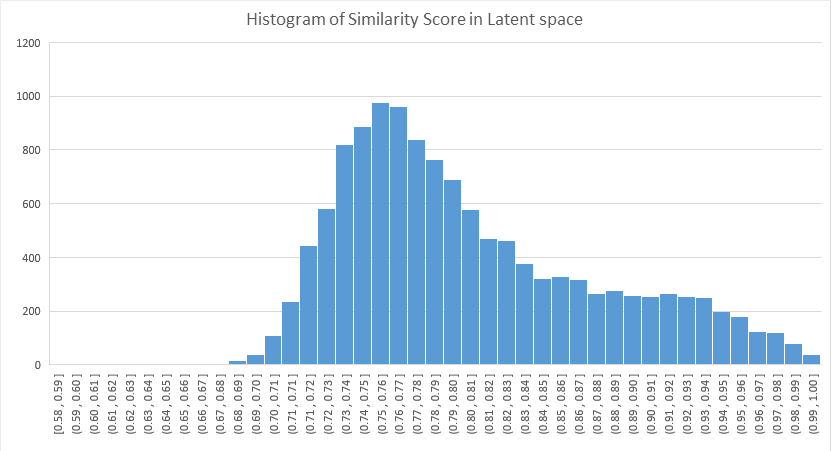
\includegraphics[width=0.8\textwidth]{img/semi-experiment/cosine_sim_histogram}
	\caption{Histogram of Cosine Similarity score}
	\label{fig:score_hist}
\end{figure}

Figure \ref{fig:score_hist} counts the occurence of similarity score over all sampled unlabeled patches. We took those samples with similarity score between 0.87 and 0.96 (sim $\in$ [0.87, 0.96]), and we assign the label of the annotated samples with highest similarity score. Figure \ref{fig:patches_noisy_mask} showed some examples of noisy labels assigned using this method.	

\begin{figure}[h]
	\centering
	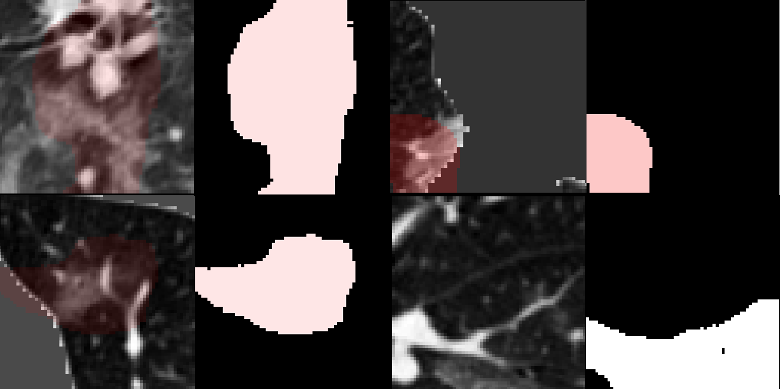
\includegraphics[width=0.8\textwidth]{img/semi-experiment/fake_assign_example}
	\caption{Example patches and noisy masks}
	\label{fig:patches_noisy_mask}
\end{figure}
\subsection{Mean teacher training}



%%%%%%%%%%%%%%%%%%%%%%%%%%%%%%%%%%%%
\chapter{Discussion and conclusion}

\section{Conclusion}
Medical segmentation on some less desired datasets in medical imaging domain focus on giving good prediction accuracy using a small amount of labelled training samples and with or without the help of non-labelled dataset. The studies in this field brings lots of benefits in the medical domain when small amount of training samples is a common scenario facing with limited resource or rarity of disease.\\

In this project, we conducted our research on the fast changing of Covid-19 data and focused our attention on segmentation tasks. We covered the two typical small sample segmentation in the project. First we perform transfer learning that we fine tuned the model to deal with the issue of the lack of data. One aspect of our work on transfer learning is that we evaluated the model using the SVCCA tool which gives us a sneak of intuition on the transfer learning process for segmentation tasks.\\

We further covered the case when a larger sets of unlabelled data is available -- Semi-supervise learning that we build a pipeline of transfer learning, psuedo-labling and mean-teacher training to improve the training process.

\section{Future work}
On hindsight, there are several improvements this work can be explored. First of all, researchers kept exploring the explainability of Neural Networks, especially in the medical imaging domain. For classification tasks given the segmentation mask, the Class Activation Map can be used to guide a better attention during network training \cite{Ouyang_2020}. Second, if future public dataset contains the follow-up CT scans of patients over a period of time, potential way for medical segmentation is to segment the infection area and perform image registration so that we can analyze the growing and absorption of infection area to better guide the clinical process.
%%%%%%%%%%%%%%%%%%%%%%%%%%%%%%%%%%%%
\chapter{Appendix A: Ethics Checklist}
This project does not involve direct human participant, while uses personal data from BraTs19 competition collected by Center for Biomedical Image Computing \& Analytics (CBICA). Furthermore, the CBICA dataset used in this project were directly downloaded from the competition. This project only uses the MRI image offered by the competition while it also offering anonymised data about the age and survival of patients. Moreover, although the dataset is officially public, we made sure that we had all the necessary authorizations to use it, and we strictly follow the BCS code and IET rules of conduct.\\

\centering
\begin{tabular}{|p{350pt}|l|c|c|}
    \hline 
    &Yes&No\\
    \hline  
    Section 1: HUMAN EMBRYOS/FOETUSES& & \\
    \hline 
    Does your project involve Human Embryonic Stem Cells?& & X\\
    \hline
    Does your project involve the use of human embryos? &&X\\
    \hline
    Does your project involve the use of human foetal tissues / cells?&&X\\
    \hline
    Section 2: HUMANS &&\\
    \hline
    Does your project involve human participants? &&X\\
    \hline
    Section 3: HUMAN CELLS / TISSUES &&\\
    \hline
    Does your project involve human cells or tissues? (Other than from Human Embryos/Foetuses i.e. Section 1)? &&X\\
    \hline
    Section 4: PROTECTION OF PERSONAL DATA &&\\
    \hline
    Does it involve the collection and/or processing of sensitive personal data (e.g.health, sexual lifestyle, ethnicity, political opinion, religious or philosophical conviction)? &X&\\
    \hline
    Does it involve processing of genetic information? &&X\\
    \hline
    Does it involve tracking or observation of participants? It should be noted that this issue is not limited to surveillance or localization data. It also applies to Wan data such as IP address, MACs, cookies etc. &&X\\
    \hline
    Does your project involve further processing of previously collected personal data (secondary use)? For example Does your project involve merging existing datasets? &&X\\
    \hline
    Section 5: ANIMALS &&\\
    \hline
    Does your project involve animals? &&X\\
    \hline
    Section 6: DEVELOPING COUNTRIES &&\\
    \hline
    Does your project involve developing countries? &&X\\
    \hline
    If your project involves low and/or lower-middle income countries, are any benefitsharing actions planned? &&X\\
    \hline
    Could the situation in the country put the individuals taking part in the project at risk? &&X\\
    \hline
    Section 7: ENVIRONMENTAL PROTECTION AND SAFETY &&\\
    \hline
    Does your project involve the use of elements that may cause harm to the environment, animals or plants? &&X\\
    \hline
    Does your project deal with endangered fauna and/or flora /protected areas? &&X\\
    \hline
    Does your project involve the use of elements that may cause harm to humans, including project staff? &&X\\
    \hline
    Does your project involve other harmful materials or equipment, e.g. high-powered laser systems? &&X\\
    \hline
\end{tabular}

\centering
\begin{tabular}{|p{350pt}|l|c|c|}
    \hline 
    Section 8: DUAL USE &&\\
    \hline
    Does your project have the potential for military applications? &&X\\
    \hline
    Does your project have an exclusive civilian application focus? &&X\\
    \hline
    Will your project use or produce goods or information that will require export licenses in accordance with legislation on dual use items? &&X\\
    \hline
    Does your project affect current standards in military ethics e.g., global ban on weapons of mass destruction, issues of proportionality, discrimination of combatants and accountability in drone and autonomous robotics developments, incendiary or laser weapons? &&X\\
    \hline
    Section 9: MISUSE &&\\
    \hline
    Does your project have the potential for malevolent/criminal/terrorist abuse? &&X\\
    \hline
    Does your project involve information on/or the use of biological-, chemical-, nuclear/radiological-security sensitive materials and explosives, and means of their delivery? &&X\\
    \hline
    Does your project involve the development of technologies or the creation of information that could have severe negative impacts on human rights standards (e.g.privacy, stigmatization, discrimination), if misapplied? &&X\\
    \hline
    Does your project have the potential for terrorist or criminal abuse e.g. infrastructural vulnerability studies, cybersecurity related project? &&X\\
    \hline
    Section 10: LEGAL ISSUES &&\\
    \hline
    Will your project use or produce software for which there are copyright licensing implications? &&X\\
    \hline
    Will your project use or produce goods or information for which there are data protection, or other legal implications? &&X\\
    \hline
    Section 11: OTHER ETHICS ISSUES &&\\
    \hline
    Are there any other ethics issues that should be taken into consideration? &&X\\
    \hline
\end{tabular}



%%%%%%%%%%%%%%%%%%%%%%%%%%%%%%%%%%%%
\chapter{Appendix}


%% bibliography
\bibliographystyle{IEEEtran}
\bibliography{ref.bib}


\end{document}
